% ------------------------------------------------------------------------------
% layout
\documentclass [twoside]{scrreprt}                % [] 10pt|11pt|12pt font size, default 10pt
	  \KOMAoptions{paper=a4}

% encoding stuff
\usepackage [utf8]{inputenc}
\usepackage [T1]{fontenc}                         % fuer korrekte trennung deutscher umlaute, scharf-s etc.


% figures
\usepackage {pgf}                                 % includepgf for bitmaps
\usepackage {epsfig}
\usepackage {psfrag}                              % replacing strings in eps files
%\usepackage [bf,small]{caption}                   % caption style
\usepackage {ifpdf}
%\ifpdf
    \usepackage{graphicx}
    \usepackage{epstopdf}
    %\DeclareGraphicsRule{.eps}{pdf}{.pdf}{`epstopdf #1}
    \pdfcompresslevel=9
%\else
  %  \usepackage {graphicx}
%\fi

\usepackage {subfig}                              % subfigures a) b)...
%\usepackage {floatflt}                           % packages supporting in-text floats
%\usepackage {wrapfig}                            % another one
%\usepackage {picins}                             % another one
%\usepackage{timing}                              % deprecated use, use below!
\usepackage{tikz-timing}                          % timing diagrams
\usepackage{sidecap}

\usepackage{listings}
\lstset{
    frameround=fttt,
    language=C,
    %numbers=left,
    breaklines=true,
    keywordstyle=\color{red}\bfseries, 
    basicstyle=\ttfamily,
    numberstyle=\color{black}
    }
\lstMakeShortInline[columns=fixed]|


% tables
\usepackage{multirow}                             % col- and rowspan...
\usepackage{booktabs}                             % professional table layout


% math
\usepackage{bbm}                                  % black board style, (e.g. \mathbbm{R})
\usepackage{amssymb}
\usepackage{amsmath}                              % e.g. \nobreakslash- for non-breakable hyphens
\usepackage{bbold}
\usepackage{amsfonts}
\usepackage{units}

% text
\usepackage {latexsym}                            % additional symbols
%\usepackage{lmodern}                              % latin modern
\usepackage [english,ngerman]{babel}              % language (change via "\selectlanguage{english}")
%\usepackage[colorlinks=true,pdftex=true,linkcolor=black,citecolor=black,urlcolor=blue,plainpages=false,pdfpagelabels]{hyperref}
\usepackage[colorlinks=true,linkcolor=black,citecolor=black,filecolor=black,urlcolor=black,plainpages=false,pdfpagelabels,breaklinks=true]{hyperref}
%\usepackage[all]{hypcap}                          % links to figures point to upper border (not caption)
\usepackage{breakurl}
\usepackage{hyphenat}
\usepackage[normalem]{ulem}                       % underline text...
\usepackage{listings}                            % source/code listings
\usepackage[plain]{algorithm}
\usepackage{algorithmicx}                        % pseudo code
\usepackage{algpseudocode}                       % pseudo code
\usepackage{units}                               % \unit[123]{U}
\usepackage{mdwlist}                             % dichtere itemize* etc.
\usepackage{paralist}                            % inline Listen
\usepackage{natbib}


% list of abbreviations, index
\usepackage{nomencl}
    \let\abbrev\nomenclature
    \renewcommand{\nomname}{List of Abbreviations}
    \setlength{\nomlabelwidth}{.25\hsize}
    \renewcommand{\nomlabel}[1]{#1 \dotfill}
    \setlength{\nomitemsep}{-\parsep}
    %\makeglossary
    \makenomenclature
    \newcommand{\markup}[1]{\uline{#1}}
\usepackage{makeidx}                              % index of key words
    \makeindex


% layout
\usepackage{xargs}                      % Use more than one optional parameter in a new commands

\usepackage[colorinlistoftodos,prependcaption,textsize=tiny]{todonotes}
\newcommandx{\add}[2][1=]{\todo[inline,#1]{#2}}
\newcommandx{\unsure}[2][1=]{\todo[linecolor=red,backgroundcolor=red!25,bordercolor=red,#1]{#2}}
\newcommandx{\change}[2][1=]{\todo[linecolor=blue,backgroundcolor=blue!25,bordercolor=blue,#1]{#2}}
\newcommandx{\info}[2][1=]{\todo[linecolor=OliveGreen,backgroundcolor=OliveGreen!25,bordercolor=OliveGreen,#1]{#2}}
\newcommandx{\improvement}[2][1=]{\todo[linecolor=Plum,backgroundcolor=Plum!25,bordercolor=Plum,#1]{#2}}
\newcommandx{\thiswillnotshow}[2][1=]{\todo[disable,#1]{#2}}
%\usepackage{stfloats}
%\usepackage{dblfloatfix}
\usepackage{fixltx2e}
%\usepackage {afterpage}                          % \afterpage{xyz} executes xyz after current page is finished
%\usepackage {flafter}                            % no object before definition
%\usepackage {float}                              % Here(!!!) placement option
% ------------------------------------------------------------------------------


% source aliases
\newcommand{\thesisTitle}{Bachelor Thesis}
\newcommand{\thesisTitleGerman}{German Title}
\newcommand{\thesisAuthor}{Arthur Heimbrecht}
\newcommand{\thesisAuthorBornIn}{Speyer}



% hypenation (englisch)
\selectlanguage{english}
\hyphenation    {HAGEN HASTE HANNEE Bert-schin-ger Maass ma-xi-mum SoftHASTE
neu-ron pre-synaptic post-synaptic}

% hypenation (deutsch)
\selectlanguage{ngerman}
\hyphenation    {HAGEN HASTE HANNEE Bert-schin-ger Maass SoftHASTE}


\tolerance 1414
\hbadness 1414
\emergencystretch 1.5em % critical parameter!!!
%\displaywidowpenalty % avoid widows after math displays
\raggedbottom % should be default anyway
%\clubpenalty = 10000
%\widowpenalty = 10000
%\hfuzz 0.3pt
%\vfuzz


%\renewcommand{\bottomfraction} {0.70} % max fraction of page for floats at bottom
%\renewcommand{\textfraction} {0.20} % min fraction of page for text
%\renewcommand{\floatpagefraction} {0.60} % min fraction of floatpage that should have floats
%\renewcommand{\dblfloatpagefraction}{0.60} % for twocolumn layout, see floatpagefraction above
%\setcounter{totalnumber} {6} % max number of floats on a single page
%\setcounter{topnumber} {6} % max number of top floats on a single page
%\setcounter{dbltopnumber}{6} % for twocolumn layout, see topnumber above
%\setcounter{bottomnumber}{6} % max number of bottom floats on a single page
% ------------------------------------------------------------------------------

\pagestyle  {empty}                               % plain, empty, headings oder myheadings.



\begin{document}

% ------------- Cover Pages ----------------------

\begin{titlepage}

\textwidth 		14cm
\textheight 		27.0cm

\evensidemargin    	-1.5cm
\oddsidemargin   	-1.5cm
\topmargin     		-3.0cm

\thispagestyle{empty}


\begin{figure}

\includegraphics{fig/cover/Publ-Cover1.eps}
%\epsfig{file=./fig/cover/Publ_Cover1.eps}% , width=\textwidth}%,height=4.5cm}
\end{figure}

\vspace*{3cm}

\hspace{5cm}
\begin{minipage}{8.2cm}
\begin{flushright}
\Large{\sf{\thesisAuthor}}
\end{flushright}
\end{minipage}


\begin{figure}[ h]

\includegraphics{fig/cover/Publ-Cover2.eps}
%\epsfig{file=./fig/cover/Publ_Cover2.eps}%,width=12.7cm}
\end{figure}

\vspace*{3mm}

\hspace{3cm}
\begin{minipage}{10.2cm}
\begin{flushright}
\Large{\sf{\thesisTitle}}
\end{flushright}

\vspace*{3mm}

\vspace*{4mm}

\begin{flushright} \Large{\sf{
%%% no = fortlaufende KIP-Nummer, wird von der Bibliothek (Tel. 8992) vergeben.
%HD-KIP-04-16
}}
\end{flushright}

\end{minipage}


\begin{figure} [b]

\includegraphics{fig/cover/Publ-Cover3.eps}
%\epsfig{file=./fig/cover/Publ_Cover3.eps}%,width=12.7cm}
\end{figure}

\end{titlepage}


\cleardoublepage
\begin{titlepage}

\begin{center}
\vspace*{2cm}
\huge{\bf{Department of Physics and Astronomy}} \\
\vspace*{0.2cm}
\LARGE{\bf{University of Heidelberg}}
\end{center}
\vspace*{10cm}
%\vfill
\large
\begin{center}
{\bf{Bachelor Thesis}} \\
\vspace*{0.2cm}
in Physics\\
\vspace*{0.2cm}
submitted by\\
\vspace*{0.2cm}
\textbf{\thesisAuthor}\\
\vspace*{0.2cm}
born in \thesisAuthorBornIn\\
\vspace*{1cm}
\textbf{TODO 2123}
\end{center}

\end{titlepage}


%\begin{titlepage}

\begin{center}
\vspace*{2cm}
\huge{\bf{Fakultät für Physik und Astronomie}} \\
\vspace*{0.2cm}
\LARGE{\bf{Ruprecht-Karls-Universität Heidelberg}}
\end{center}
\vspace*{10cm}
%\vfill
\large
\begin{center}
{\bf{Bachelorarbeit}} \\
\vspace*{0.2cm}
im Studiengang Physik\\
\vspace*{0.2cm}
vorgelegt von\\
\vspace*{0.2cm}
\textbf{\thesisAuthor}\\
\vspace*{0.2cm}
geboren in \thesisAuthorBornIn\\
\vspace*{1cm}
\textbf{TODO 2123}
\end{center}

\end{titlepage}



\cleardoublepage
\begin{titlepage}

\begin{center}
\vspace*{2cm}
\huge{\textbf{\thesisTitle}}\\
%\huge{\bf}\\
\end{center}
\vspace*{10cm}
%\vfill
\large
\begin{center}
{\bf This Bachelor Thesis has been carried out by \thesisAuthor{} at the} \\
\vspace*{0.2cm}
{\sc Kirchhoff Institute for Physics\\

\vspace*{0.2cm}
Ruprecht-Karls-Universität Heidelberg\\}
\vspace*{0.2cm}
{\bf under the supervision of}\\
\vspace*{0.2cm}
{\bf Prof. Dr. Karlheinz Meier}\\
\end{center}

\clearpage

\vspace*{15cm}
\begin{center}
%For someone.
\end{center}


\end{titlepage}


%\begin{titlepage}

\begin{center}
\vspace*{2cm}
\huge{\textbf{\thesisTitleGerman}}\\
%\huge{\bf}\\
\end{center}
\vspace*{10cm}
%\vfill
\large
\begin{center}
{\bf Diese Bachelorarbeit wurde von \thesisAuthor{} ausgeführt am} \\
\vspace*{0.2cm}
{\sc Kirchhoff-Institut für Physik\\

\vspace*{0.2cm}
Ruprecht-Karls-Universität Heidelberg\\}
\vspace*{0.2cm}
{\bf unter der Betreuung von}\\
\vspace*{0.2cm}
{\bf Prof. Dr. Karlheinz Meier}\\
\end{center}

\clearpage

\vspace*{15cm}
\begin{center}
%For someone.
\end{center}


\end{titlepage}



%-------------------------------------------------






% and now in englisch!
\selectlanguage{english}





% ------------- Abstract -------------------------

\cleardoublepage

\pagestyle{plain}

\setcounter{page}{1}
\pagenumbering{Roman}

\begin{abstract}
\begin{center}
\textbf{\thesisTitle}
\end{center}

As part of the Human Brain Project, BrainScaleS is a unique project on many levels. This includes a processor solely used by the HICANN-DLS, which manages synaptic weights for every neuron built into one of the many wafers. To accelerate the speed at which this so called plasticity processor unit (PPU) computes all synaptic weights of every neuron used, the processor has an extended instruction set architecture (ISA) that supports vector registers and single input multiple data (SIMD).
This report deals with the task of adding built-in functions to an existing back-end of GCC, specifically the one used by the PPU, in order to extend the already implemented set of functions according to the users needs.
\end{abstract}


%-------------------------------------------------




% ------------- Table of Contents ----------------

\cleardoublepage
\setcounter{tocdepth}{3}
\tableofcontents

%-------------------------------------------------






% ------------- Chapters -------------------------

\cleardoublepage

\pagestyle{headings}

\setcounter{page}{1}
\pagenumbering{arabic}



%%% INCLUDES %%%%%%%%%%%%%%%%%%%%%%%%%%
% introduction
\chapter{Introduction}
\label{chapter:introduction}

Neuromorphic computing has developed into a popular scientific field throughout the last years and finds more and more applications and implementations in science and industry, e.g.~\cite{6905473}.
These systems already show advantages over traditional computer architectures, like the von-Neumann architecture, in specific applications and continue to improve.
In its current generation, neural networks abandon discrete time steps and states, but gain more computational power~\cite{Maass19971659}.
They use spikes and continuous time scales that resemble nature more closely and allow for efficient implementations as analog hardware which offers high performance at low energy consumption~\cite{NIPS2015_5862}.
Still, new architectures also require novel styles of programming~\cite{Amir2013CognitiveCP} and users need to adapt to these.
This can be a hurdle for many users when developing new experiments, that initially take a significant amount of time. 
\\
\\
One example for this is the current way of programming for the plasticity processing unit of the \ac{HICANN-DLS}. 
The \ac{HICANN-DLS} is a small scale system that features analog emulation of neurons and synapses in networks~\cite{PPU}.
The \ac{PPU}, as part of \ac{HICANN-DLS}, can be used for implementing plasticity rules for such networks.
It resembles a traditional processor architecture, which was modified for this task.
Implementing such plasticity rules differs from conventional high-level programming styles. 
When creating code for the \ac{PPU}, users are partially pushed back to the origins of computing;
instead of assigning values like |d = a + b|, one must first read the variables from memory, then operate on their values and finally write back the result to memory.
Therefore coding for the \ac{PPU} works on a low level and brings new challenges to users, that are already challenged by neuromorphic programming.

Ultimately, the more a system abandons conventional elements of programming, the more challenges emerge from this.
Although experienced programmers can create highly efficient code like this, normal users will not be familiar with this.
This can cause fewer users to take the initiative of writing code for such systems, but also can code get confusing, hard to debug and even inefficient.
\\
\\
Compilers usually save users from these problems by offering high-level languages.
Over decades compilers have been developed and became a standard tool for programmers.
At the same time compilers became more and more of a black box that transforms a program into an executable file.
For this reason it may be difficult for some users to abandon their convenience and go back to low-level programming.

Though the \ac{PPU} is not completely without compiler support, its distinct features are only usable on a low level.
As these features are necessary to implement plasticity rules on the \ac{HICANN-DLS}, this can easily cause inconveniences for users.
Users repeatedly have to mix high-level and low-level code, which is an atypical style of programming.
It can cause different problems, as users have to adapt to this and, in the beginning, likely create bugged or inefficient programs.
As performance is important for neuromorphic programming, users may need an unreasonable amount of time and work to achieve simple results with this.
\\
\begin{wrapfigure}{R}{0.5\textwidth}
\captionsetup{format=plain, indention=.6cm, labelsep=newline,singlelinecheck=false}
    \centering
    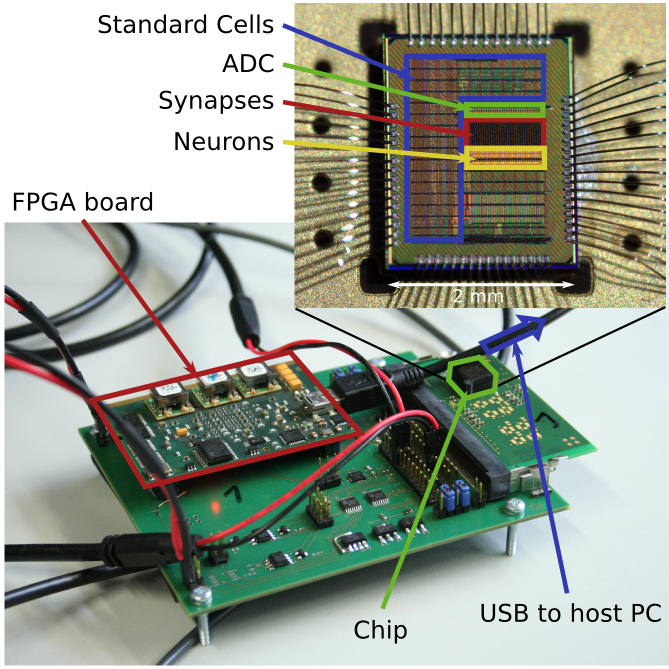
\includegraphics[width=0.4\textwidth]{pictures/Fig1.png}
    \caption{\label{fig:dlsboard} Set-Up of a \ac{HICANN-DLS} Test System (from~\citeauthor{PPU})}
\end{wrapfigure}
\\
Until now full compiler support does not exist for the \ac{PPU} because of its modified processor architecture, which was developed solely for neuromorphic hardware.
It offers a partly customized instruction set that is optimized for its applications.
\\
The \ac{HICANN-DLS} already is an experimental platform, which is used by several users, even though of \ac{PPU}-related challenges.
Applications like in-the-loop training or \ac{STDP} have been developed and mostly do not involve the \ac{PPU} .
Even when taking the effort of learning to code for the \ac{PPU}, users are constantly challenged by missing programming features such as creating parameterized functions.
This leads to repetitive code or difficulties when integrating calibration into experiment-related code.

Offering more tools for \ac{PPU} programs could reduce the effort of developing for the \ac{PPU}, while at the same time increasing capabilities of programs.
Besides allowing full high-level programming, compiler support could also offer tools like code optimization and debugging features.
At some point compiler support may also facilitate automatic code generation as a prerequisite for implementation of very high-level languages.
Users then could create plasticity rules in existing program environments from where code is translated into \ac{PPU} programs.
This creates the need for optimization of \ac{PPU} code, like those built into virtually every compiler.
\\
\\
This thesis will focus on achieving aforementioned compiler support and briefly explain the process itself.
As fundamental knowledge of both, processors and compilers, is needed along the way, the second chapter will start with a very basic introduction to both topics.
This involves basic information about the \ac{PPU}, as well as the \ac{GCC}, and should explain the basic concepts to an extend which is sufficient.
Afterwards, the process of extending the compiler is explained, followed by a presentation of results as well as first test cases.
The thesis will conclude in a resume and give an outlook to future applications and development of the compiler and the \ac{PPU}.



    \tcbset
    {enhanced,colframe=blue!70!black,colback=white!50!blue,colupper=red!50!black,
    fonttitle=\bfseries,nobeforeafter,center title, noparskip}
    \noindent{\begin{minipage}{\textwidth}
        \begin{minipage}[c][][c]{0.25\textwidth}
            \begin{tcolorbox}[tcbox raise base, width=\linewidth, remember as=cp, enhanced, watermark text=Compiler]
                \begin{tcolorbox}[enhanced, breakable, noparskip,opacityframe=0.0, opacityback=0.0, height=2cm, width=\linewidth]
                \end{tcolorbox}
                \begin{tcolorbox}[enhanced, breakable, noparskip,opacityframe=0.0, opacityback=0.0, height=1cm, width=\linewidth]
                \end{tcolorbox}
                \begin{tcolorbox}[enhanced, breakable, noparskip,opacityframe=0.0, opacityback=0.0, height=1.5cm, width=\linewidth]
                \end{tcolorbox}
            \end{tcolorbox}
            \begin{tikzpicture}[overlay,remember picture,line width=1mm]
                \draw[->, shorten >=-1.5mm] ($(cp.north)+(0,1)$) -- node [left] {program code} (cp.north);
                \draw[->] (cp.south) -- node [left] {machine files} ($(cp.south)+(0,-1)$);
            \end{tikzpicture}
        \end{minipage}
\end{minipage}}


\chapter{Extending the \ac{GCC} Back-End}
\label{chapter:extbackend}
The previous chapter dealt with processors, the \ac{PPU}, compilers and \ac{GCC}, which was preparation for this chapter.
This chapter will now emphasize on the task of extending the \ac{GCC} back-end.
There is a number of files, which will be systematically edited and referenced as they are important parts of the \ac{rs/6000} back-end and are changed in the process of extending the back-end. 
\begin{description}
    \item[rs6000.md] is the machine description of the back-end in general and contains insn definitions for all scalar functions
    \item[rs6000.h] is a header file which contains macros and declarations for registers
    \item[rs6000.c] is the source file which implements the back-end's functions
    \item[rs6000.opt] lists the options and flags for the target
    \item[rs6000-builtins.def] contains the definitions of intrinsics
    \item[rs6000-cpus.def] lists sub-targets that belong to the \ac{rs/6000} family
    \item[rs6000-c.c] links built-ins and overloaded built-ins
    \item[rs6000-opts.h] contains a set of enumerations that represent option values for the back-end
    \item[rs6000-protos.h] makes functions in |rs6000.c| globally available
    \item[rs6000-tables.opt] lists values to a processor enumeration
    \item[driver-rs6000.c] a collection of driver details for different targets
    \item[ppc-asm.h] sets macros for the use of |asm|
    \item[s2pp.md] is a new machine description of \ac{s2pp} and contains insn definitions
    \item[s2pp.h] is the header file that defines aliases for built-ins
    \item[constraints.md] contains definitions of constraints
    \item[predicates.md] contains definitions of predicates
    \item[vector.md] defines general vector insns
    \item[sysv4.h] initializes a variety of option flags and sets default values
    \item[t-fprules] sets soft-float as default for certain targets
\end{description}

It is recommended to have chapter 5 of the \textbf{nux manual}~\citep[ch.~5]{nuxmanual} at hand, as it contains an overview of existing \ac{s2pp} vector instructions.

Before extending the \ac{GCC} back-end a few things must be stated:

Due to the limited documentation of the back-end itself, one must rely on comments in code and the \textbf{\ac{GCC} internals manual}~\citep{GCCint} 
As a full implementation for a vector extension already exists, the AltiVec extension should be used as a guideline for a new extensions~\cite{AltiVec}. 
Still, it should be avoided to change exiting code as much as possible.
Code is often referred to from different places in the back-end and modifying existing code can therefore easily lead to compiler errors.
Especially since the back-end is not extended completely right away but rather step by step.
This applies particularly to functions that are implemented for AltiVec only.
It is recommended to rather duplicate functions and distinguish them, before they are called.
This will make it easier to find bugs, as usually the function that generates an error is indicated in the error message.
Also, there do exist enough differences between these two vector extensions, that combining functions would not save work.

It will therefore occasionally be pointed out when functions or other code can be inherited from AltiVec and which modifications are needed.

\section{Adding the s2pp Option Flag and nux Target}
Extending the rs6000 back-end starts by adding the |nux| processor to the list of targets and also including mandatory flags with this.
Ideally the user only has to add the flag |-mcpu=nux| when compiling, in order to produce machine code for the nux.
The flags which have to be set when using the nux are:
\begin{description}
        \lstitem{-msdata=none}
        disables the use of a \textbf{small data section} which is like a data section but has a register constantly referring to it and thus has faster access than the normal data section. Globals, statics and small variables that are often used are preferably stored there. It is turned off because the base pointer is not initialized by the linker and the effect of a small data section would likely be small for the \ac{PPU}~\cite{nuxmanual, ibmsda, websda}.
        \lstitem{-mstrict-align}
        aligns all variables in memory which means that a variable always starts at a memory address which is a multiple of its size. E.g. a vector has always an address that is dividable by 16 bytes or 128 bits. Memory management is far easier for aligned variables.
        \lstitem{-msoft-float}
        tells the compiler that there is no FPU and all floating point operations have to simulated by software.
        \lstitem{-mno-relocatable}
        states that the program code has a fixed memory address that may not be altered. Relocatable code is not needed as the \ac{PPU} runs only one program that is loaded into memory and uses no environment on top.
\end{description}

But first there should be an \textbf{option flag} that activates nux' \ac{VE} like |-maltivec| does for the AltiVec \ac{VE}.
The name for this new option flag will be |-ms2pp| and it will define an option mask along with it.
In |rs6000.opt| and we simply need to add:
\begin{lstlisting}
ms2pp
Target Report Mask(S2PP) Var(rs6000_isa_flags)
Use s2pp instructions
\end{lstlisting}
This adds |ms2pp| to the list of option flags and the next lines defines a macro, that is associated with it.
|Target| means that the option is target specific, therefore only certain architectures support the option flag.
|Report| means that the option is printed when |-fverbose-asm| is is set.
|Mask(S2PP)| initializes a bitmask, that is available through |OPTION_MASK_S2PP|.
That macro is attached to |rs6000_isa_flags|, which is specified by |Var|.
It simultaneously specifies a macro |TARGET_S2PP| that is set to |1|~\citep[ch.~8]{GCCint}.

This needs also specification of 
\begin{lstlisting}
#define MASK_S2PP OPTION_MASK_S2PP
\end{lstlisting}
in |rs6000.h| as macros with |MASK_| are a standard from earlier versions of \ac{GCC}.

Although this option flag shall later enable \ac{s2pp} support, it needs the aforementioned flags as well, to compile nux programs.
For this reason exists a processor type which combines those flags.
There exist several lists that contain available targets and nux shall be included.
First an inline assembly (see section~\ref{section:asm}) flag is created, which tells the assembler which system architecture is used.
As nux is based on POWER7, one can copy the flag |-mpower7| in |driver-rs6000.def|:
    \begin{lstlisting}[caption=\tt rs6000.h]
    #define ASM_CPU_SPEC \
        ...
        %{mcpu=power7: %(asm_cpu_power7)} \
        ...
        %{mcpu=nux: %(asm_cpu_power7)} \
        ...
    \end{lstlisting}
    \begin{lstlisting}[caption=\tt driver-rs6000.c]
    static const struct asm_name asm_names[] = {
        ...
        { "power7",   "%(asm_cpu_power7)" },
        ...
        { "nux",  "%(asm_cpu_power7)" },
        ...
    \end{lstlisting}
This will set the assembler |-mpower7| when using |-mcpu=nux|.

The nux target should also be recognized by preceding phases of the compiler and set option flags accordingly.
These options flags can be set in |rs6000-cpus.def|.

\begin{lstlisting}
...
RS6000_CPU ("nux", PROCESSOR_POWER7, MASK_SOFT_FLOAT | MASK_S2PP | MASK_STRICT_ALIGN | !MASK_RELOCATABLE)
\end{lstlisting}

This uses the macro |RS6000_CPU (NAME, CPU, FLAGS)| and adds |nux| to the |processor_target_table[]|.
Since option flags usually set masks, one can set the respective masks directly.
The masks will tell the compiler that the processor is a POWER7 architecture and uses |soft-float|, |strict-align| and |no-relocatable|(negated relocatable) as well as the new s2pp mask.

It is not possible, to set the |-msdata=none| flag before since the |-msdata| flag is initialized differently.
Also since it is not simply set ``on'' or ``off'' but accepts several values, it is handled in |sysv4.h|.
|rs6000_sdata| will be set according to the string that follows |-msdata=|.
\begin{lstlisting}
#define SUBTARGET_OVERRIDE_OPTIONS                          \
...
  if (rs6000_sdata_name)                                    \
     {                                                      \
       if (!strcmp (rs6000_sdata_name, "none"))             \
     rs6000_sdata = SDATA_NONE;                             \
     ...
       else                                                 \
     error ("bad value for -msdata=%s", rs6000_sdata_name); \
     }                                                      \
  else if (OPTION_MASK_S2PP                                 \
          && OPTION_MASK_SOFT_FLOAT                         \
          && OPTION_MASK_STRICT_ALIGN                       \
          && !OPTION_MASK_RELOCATABLE)                      \
     {                                                      \
     rs6000_sdata = SDATA_NONE;                             \
     rs6000_sdata_name = "none";                            \
     }                                                      \
  else if (DEFAULT_ABI == ABI_V4)                           \
...
)\todo{looose this!!!!!!!!!!!!!!!!!!!!!!}
\end{lstlisting}

It is not possible to detect in this file, if the nux flag is set.
It therefore needs a little workaround that helps setting the value of |rs6000_sdata|.
If |-msdata| is not set, i.e. only |-mcpu=nux| is set, the compiler will use |if|-clauses that determine which value is assigned to |rs6000_sdata|.
It is possible, to add a case that checks for all flags, that are set by |-mcpu=nux| and set |rs6000_sdata| to |SDATA_NONE| if this applies.
Hence the target options will set |rs6000_sdata| to |SDATA_NONE|.

There exists a case for which this condition applies even when |nux| is not set as target, but all flags are set by hand.
If one chooses an explicit value for |-msdata|, this case does not apply though and the value of |-msdata| is set accordingly.

This is not an ideal solution, but a trade-off with as few side effects as possible.
\\
\\
Already this would allow for the use of |-mcpu=nux| as target and |-ms2pp| as option flag.
But since the flags we used are basically mandatory to the \ac{s2pp} extension, the compiler should check for these flags before starting compilation.
First though for each flag needs a macro, which the back-end can identify.
This is done in |rs6000-c.c| where \textbf{global macros} can be defined:
\begin{lstlisting}
rs6000_target_modify_macros (bool define_p, HOST_WIDE_INT flags,
                 HOST_WIDE_INT bu_mask)
{...
  if ((flags & OPTION_MASK_S2PP) != 0)
   rs6000_define_or_undefine_macro (define_p, "__S2PP__");
  if ((flags & OPTION_MASK_STRICT_ALIGN) != 0)
   rs6000_define_or_undefine_macro (define_p, "_STRICT_ALIGN");
  if ((flags & OPTION_MASK_RELOCATABLE) != 0)
   rs6000_define_or_undefine_macro (define_p, "_RELOCATABLE");
  if (rs6000_sdata != SDATA_NONE)
   rs6000_define_or_undefine_macro (define_p, "_SDATA");
   ...}
\end{lstlisting}

If |flags| and the respective option masks are set, |rs6000_define_or_undefine_macro| will define a macro that is specified by the second argument.
Whether a macro is defined or undefined depends on the boolean |define_p|, which is set by the compiler.

These new macros can be used to check if flags are set.
This needs a new file, that will also be needed later on as the \textbf{\ac{s2pp} header file}.
|s2pp,h| must be indexed in |gcc/config.gcc| under |extra_headers|.
\begin{lstlisting}
...
powerpc*-*-*)
    cpu_type=rs6000
    extra_headers="ppc-asm.h altivec.h spe.h ppu_intrinsics.h paired.h spu2vmx.h vec_types.h si2vmx.h htmintrin.h htmxlintrin.h s2pp.h"
    need_64bit_hwint=yes
    case x$with_cpu in
    xpowerpc64|xdefault64|x6[23]0|x970|xG5|xpower[345678]|xpower6x|xrs64a|xcell|xa2|xe500mc64|xe5500|Xe6500)
    cpu_is_64bit=yes
    ;;
    esac
    extra_options="${extra_options} g.opt fused-madd.opt rs6000/rs6000-tables.opt"
    ;;
...
\end{lstlisting}
This is done, so \ac{GCC} invokes the header file, as it is not referenced elsewhere.

|s2pp.h| can now be used to check the compiler flags.
\begin{lstlisting}
/* _S2PP_H */
#ifndef _S2PP_H
#define _S2PP_H 1

#if !defined(__S2PP__)
#error Use the "-ms2pp" flag to enable s2pp support
#endif
#if !defined(_SOFT_FLOAT)
#error Use the "-msoft-float" flag to enable s2pp support
#endif
#if !defined(_STRICT_ALIGN)
#error Use the "-mstrict-align" flag to enable s2pp support
#endif
#if defined(_RELOCATABLE)
#error Use the "-mno-relocatable" flag to enable s2pp support
#endif
#if defined(_SDATA)
#error Use the "-msdata=none" flag to enable s2pp support
#endif
...
\end{lstlisting}

If for example |__S2PP__| is not defined but |s2pp.h| included, the compiler will emit an error that tells the user to set the target flag.
Since hard floats are not supported on |nux| regardless of |s2pp.h|, nux can be added to the list of soft-float processors in |t-fprules|.
\begin{lstlisting}
SOFT_FLOAT_CPUS = e300c2 401 403 405 440 464 476 ec603e 801 821 823 860 nux
\end{lstlisting}

\section{Creating Macros}
Since the preliminary requirements are now met, the back-end needs a \textbf{{\tt vector} attribute} for specifying vectors in program code.
Attributes are used to specify various variables and can be used for example to control alignment~\citep[ch.~16.19]{GCCint}.

First a new vector unit is needed.
It will be called |VECTOR_S2PP| and added to the enumeration |rs6000_vector| in |rs6000-opts.h|.
\begin{lstlisting}
enum rs6000_vector {
      VECTOR_NONE,          /* Type is not  a vector or not supported */
      VECTOR_ALTIVEC,       /* Use altivec for vector processing */
      VECTOR_VSX,           /* Use VSX for vector processing */
      VECTOR_P8_VECTOR,     /* Use ISA 2.07 VSX for vector processing */
      VECTOR_PAIRED,        /* Use paired floating point for vectors */
      VECTOR_SPE,           /* Use SPE for vector processing */
      VECTOR_S2PP,          /* Use s2pp for vector processing */ //s2pp-mark
      VECTOR_OTHER          /* Some other vector unit */
};
\end{lstlisting}

To put this to use, it needs macros in |rs6000.h| which compare vector units to the newly created |VECTOR_S2PP|.
\begin{lstlisting}
...
#define VECTOR_UNIT_S2PP_P(MODE)            \
    (rs6000_vector_unit[(MODE)] == VECTOR_S2PP)
...
#define VECTOR_MEM_S2PP_P(MODE)             \
  (rs6000_vector_mem[(MODE)] == VECTOR_S2PP)
...
\end{lstlisting}

|VECTOR_UNIT_S2PP_P(MODE)| and |VECTOR_MEM_S2PP_P(MODE)| are identical as identical entries in |rs6000_vector_unit[]| and |rs6000_vector_mem[]| are created.
This is a relict from the AltiVec implementation as vector units in memory may differ in certain cases. 

Checking for specific \textbf{vector modes}, which are supported by \ac{s2pp}, will also be added.
The nux hardware only supports two types of vectors which are vectors with byte elements (V16QI) and vectors with half-word elements (V8HI).
\begin{lstlisting}
#define S2PP_VECTOR_MODE(MODE)        \
         ((MODE) == V16QImode)        \
          ||  (MODE) == V8HImode)
\end{lstlisting}

Some uses of |TARGET_ALTIVEC| must now be accompanied by |TARGET_S2PP| to handle vectors correctly.
There exist five such cases:

|rs6000_builtin_vectorization_cost|, |rs6000_special_adjust_field_align_p| and |expand_block_clear| handle alignment of vectors.
\textbf{Alignment} refers to the position of data blocks in memory; 16-bit alignment means that variables may only start at addresses that represent multiples of 16 bits.
AltiVec vectors and s2pp are aligned the same way and it is desirable to reduce misalignment of 128-bit vectors to a minimum.

|rs6000_common_init_builtins| initializes common built-ins and is needed by all extensions that use built-ins (see section~\ref{sec:builtins}).
In these cases the condition can be extended for |TARGET_S2PP|.

Other conditions that will later be extended for |TARGET_S2PP| need further modification and thus are not mentioned here.

It is necessary, to do the same for |VECTOR_UNIT_S2PP_P| and other macros that have AltiVec counterparts:
In |reg_offset_addressing_ok_p| cases for |V16QImode| and |V8HImode| return false if |VECTOR_MEM_S2PP_P| or the AltiVec version apply.
In |rs6000_legitimize_reload_address| and |rs6000_legitimate_address_p| offset addresses are handled the same way they are handled for AltiVec.
In |rs6000_secondary_reload| indirect addressing is enforced.
In |print_operand| operand modifier |y| is validated for \ac{s2pp}.
|rs6000_vector_mode_supported_p| returns true if a mode is supported by \ac{s2pp}.

All of these cases handle addressing of vectors in memory which is equivalent for AltiVec and \ac{s2pp}.
It is therefore quite simple to support this for \ac{s2pp}.
\\
\\
Since vector modes and units have been established by now, it is possible to connect these in |rs6000_init_hard_regno_mode_ok|.
In case |TARGET_S2PP| is set |VECTOR_S2PP| is assigned to modes |V16QImode| and |V8HImode|.
\begin{lstlisting}
...
  if (TARGET_S2PP)
      {
      rs6000_vector_unit[V8HImode] = VECTOR_S2PP;
      rs6000_vector_mem[V8HImode] = VECTOR_S2PP;
      rs6000_vector_align[V8HImode] = align32;
      rs6000_vector_unit[V16QImode] = VECTOR_S2PP;
      rs6000_vector_mem[V16QImode] = VECTOR_S2PP;
      rs6000_vector_align[V16QImode] = align32;
      }
...
\end{lstlisting}

Preferred modes when vectorizing a non-vector mode in |rs6000_preferred_simd_mode| can be set.
\begin{lstlisting}
...
  if (TARGET_S2PP)
    switch (mode)
        {
        case HImode:
      return V8HImode;
        case QImode:
      return V16QImode;
        default:;
        }
... 
\end{lstlisting}

It is now possible to create vector attributes, as mentioned before.
\ac{GCC} already supports a vector attribute which is also used by AltiVec.
Thus \ac{s2pp} can be added to |rs6000_attribute_table| and |rs6000_opt_masks[]| array with the same values as for AltiVec but changing the keyword.
\begin{lstlisting}
static const struct attribute_spec rs6000_attribute_table[] =
{
    /* { name, min_len, max_len, decl_req, type_req, fn_type_req, handler,
         affects_type_identity } */
    { "altivec",   1, 1, false, true,  false, rs6000_handle_altivec_attribute,
      false },
    { "s2pp",   1, 1, false, true,  false, rs6000_handle_s2pp_attribute,
      false },
  ...}
struct rs6000_opt_mask {
  const char *name;     /* option name */
  HOST_WIDE_INT mask;       /* mask to set */
  bool invert;          /* invert sense of mask */
  bool valid_target;        /* option is a target option */
};

static struct rs6000_opt_mask const rs6000_opt_masks[] =
{
  { "altivec",          OPTION_MASK_ALTIVEC,        false, true  },
  ...
  { "s2pp",         OPTION_MASK_S2PP,       false, true  },
  ...}
\end{lstlisting}

The function |rs6000_handle_s2pp_attribute| is also copied from AltiVec, but stripped off unsupported vector modes.

This would make these attributes already usable but defining built-ins in |rs6000-c.c| shortens the attribute from |__vector=__attribute__((s2pp(vector__)))| to |__vector|:
\begin{lstlisting}
void
rs6000_cpu_cpp_builtins (cpp_reader *pfile)
{
  ...
  if (TARGET_S2PP){
     builtin_define ("__vector=__attribute__((s2pp(vector__)))");
     if (!flag_iso){
        builtin_define ("vector=vector");
        init_vector_keywords ();
        /* Enable context-sensitive macros.  */
        cpp_get_callbacks (pfile)->macro_to_expand = rs6000_macro_to_expand;
     }
  }
... 
\end{lstlisting}
|__vector| is then used to define |vector| in |s2pp.h|.
\begin{lstlisting}
#define vector __vector
\end{lstlisting}

At last it must be indicated to the front-end, that special attributes are handled by the back-end.
\begin{lstlisting}
static bool
rs6000_attribute_takes_identifier_p (const_tree attr_id)
{
  if (TARGET_S2PP)
    return is_attribute_p ("s2pp", attr_id);
  else
    return is_attribute_p ("altivec", attr_id);
}
\end{lstlisting}

\section{Registers}
\label{section:register}
This section will describe, how \ac{s2pp} registers are added to the back-end.
It will also add constraints and predicates (see section~\ref{sec:defineinsn}) for these registers.

There are three types of registers in the \ac{s2pp} \ac{VE}:
\begin{description}
    \item[32 vector registers] these are normal vector registers that hold vector values
    \item[1 accumulator] which is used for chaining arithmetic instructions and cannot be accessed directly
    \item[1 conditional register] which holds conditional bits and also cannot be accessed directly
\end{description}

During extension of the \ac{GCC} back-end, it becomes apparent that a reserved vector register, that is all zeros the entire time, will be necessary for some implementations of the back-end.
This is necessary since the nux instruction set does not include logical vector instructions.
Normally the instructions |XOR| and |OR| are used by the back-end to implement simple register features.
|OR| is used for moving around the content of a register, as |OR|ing the same first register to a second register will simply copy the contents of the first register.
On the other side, does |XOR|ing the same register result in writing all zeros to the return register.

Since these instructions are not available, ``nulling'' a register becomes a problem.
Therefore the first register is reserved and splatted with zeros.
Moving this register, will have the same effect as |XOR|ing a register.
As |OR| is also not available, an alternative instruction is used, which is |fxvselect|.
|fxvselect| selects either elements of the second or the third operand depending on the condition register and its forth operand~\citep[ch.~5]{nuxmanual}.
Having identical second and third operands thus will simply generate the same vector as return value.
By setting the forth operand |0|, |fxvselect| will always choose elements from the second operand.
This gives a simple work-around, as |fxvselect| also takes only one clock cycle for execution.
An alternative idea would be subtracting the same register from itself with |fxvsubm|, which also nulls the return operand.
This would take more clock cycles though and is unfavorable, as it is not clear, how often registers need to be nulled.
Ultimately it is a trade-off between having one less register at hand and possibly wasting clock cycles continuously.
In this case it is preferable to give up a single register, as the amount of nulling instructions is unknown.
At a later point in time, this could be reviewed for performance, which might overturn this decision.

It is not possible to splat zeros constantly because this would require an extra instruction to load a zero into a \ac{GPR}.
This is not possible at late stages of code generation as all registers are already allocated at that time.
\\
\\
When talking about reserved registers, one must also think about saved, call-used and fixed registers:
\begin{description}
    \item[fixed registers] serve only one purpose and are not available for allocation at all.
    \item[call-used registers] are used for returning results of functions. They are not available to general register allocation but are used when calling functions.
    \item[saved registers] are available globally and may hold values throughout function calls.
\end{description}

Usually about half of all registers are declared call-used and the other half saved.
This is done for AltiVec, as well as \acp{FPR}, but might be optimized in the future, depending on requirements of applications (e.g. are many function calls used).
\\
\\
\textbf{Register indexes} are declared in |rs6000.md|:
\begin{lstlisting}
(define_constants
  [(FIRST_GPR_REGNO     0)
...
   (LAST_GPR_REGNO      31)
   (FIRST_FPR_REGNO     32)
   (LAST_FPR_REGNO      63)
   (FIRST_S2PP_REGNO    33)
   (LAST_S2PP_REGNO     63)
   (S2PP_COND_REGNO     32)
   (S2PP_ACC_REGNO      64)
   (LR_REGNO            65)
...])
\end{lstlisting}
Each register index is a unique identifier of registers and is given in incrementing order.
Registers which may be available on the same processor must not share and index!
\ac{s2pp} reuses the reserved vector register's index 32 (this register is always null) for the conditional register and uses the free index 64 for the accumulator.
As the GPRs need the first 32 registers numbers (0-31) and there is never an FPU on nux, it is possible, to use the 32 registers normally reserved to FPRs.

It then is decided, which registers shall be used for function calls, and therefore reserved for call-use.
This is declared by macros that are assigned a register number in |rs6000.md|.
\begin{lstlisting}
/* Minimum and maximum s2pp registers used to hold arguments.  */
#define S2PP_ARG_MIN_REG (FIRST_S2PP_REGNO + 2)
#define S2PP_ARG_MAX_REG (S2PP_ARG_MIN_REG + 12)
#define S2PP_ARG_NUM_REG (S2PP_ARG_MAX_REG - S2PP_ARG_MIN_REG + 1)
...
#define S2PP_ARG_RETURN S2PP_ARG_MIN_REG
...
#define S2PP_ARG_MAX_RETURN (DEFAULT_ABI != ABI_ELFv2 ? S2PP_ARG_RETURN \
                    : (S2PP_ARG_RETURN + AGGR_ARG_NUM_REG - 1))
...

#define FUNCTION_VALUE_REGNO_P(N)                   \
  ((N) == GP_ARG_RETURN                         \
     || ((N) >= FP_ARG_RETURN && (N) <= FP_ARG_MAX_RETURN         \
         && TARGET_HARD_FLOAT && TARGET_FPRS)             \
     || ((N) >= ALTIVEC_ARG_RETURN && (N) <= ALTIVEC_ARG_MAX_RETURN   \
         && TARGET_ALTIVEC && TARGET_ALTIVEC_ABI)             \
     || ((N) >= S2PP_ARG_RETURN && (N) <= S2PP_ARG_MAX_RETURN     \
         && TARGET_S2PP)              \
     )
...
#define FUNCTION_ARG_REGNO_P(N)                     \
  ((unsigned) (N) - GP_ARG_MIN_REG < GP_ARG_NUM_REG         \
     || ((unsigned) (N) - ALTIVEC_ARG_MIN_REG < ALTIVEC_ARG_NUM_REG   \
         && TARGET_ALTIVEC && TARGET_ALTIVEC_ABI)             \
     || ((unsigned) (N) - FP_ARG_MIN_REG < FP_ARG_NUM_REG         \
         && TARGET_HARD_FLOAT && TARGET_FPRS)             \
     || ((unsigned) (N) - S2PP_ARG_MIN_REG < S2PP_ARG_NUM_REG     \
         && TARGET_S2PP)              \
     )
...
\end{lstlisting}

The only use of these macros is in the prologue and the epilogue, which will be discussed in the next section.

After all register indexes are declared, they can be specified further.
Each register type (or \textbf{register class}) needs an entry to the enumeration |reg_class| and a definition of identical register names in |REG_CLASS_NAMES|.
\begin{lstlisting}[multicols=2]
enum reg_class
{
  ...
  GENERAL_REGS,
  S2PP_C_REG,
  S2PP_REGS,
  FLOAT_REGS,
  S2PP_ACC_REG,
  ALTIVEC_REGS,
  ...
  ALL_REGS}
...
#define REG_CLASS_NAMES  \
  {                      \
  ...
  "GENERAL_REGS",        \
  "S2PP_C_REG",          \
  "S2PP_REGS",           \
  "FLOAT_REGS",          \
  "S2PP_ACC_REG",        \
  "ALTIVEC_REGS",        \
  ...
  "ALL_REGS"}
  \end{lstlisting}

Then the relation between register classes in specified in |REG_CLASS_CONTENTS|.
\begin{lstlisting}
/* GENERAL_REGS.  */                          \
{ 0xffffffff, 0x00000000, 0x00000008, 0x00020000, 0x00000000 },   \
/* S2PP_C_REG.  */                                                \
{ 0x00000000, 0x00000001, 0x00000000, 0x00000000, 0x00000000 },   \
/* S2PP_REGS.  */                                                 \
{ 0x00000000, 0xfffffffe, 0x00000000, 0x00000000, 0x00000000 },   \
/* FLOAT_REGS.  */                                                \
{ 0x00000000, 0xffffffff, 0x00000000, 0x00000000, 0x00000000 },   \
/* S2PP_ACC_REG.  */                                              \
{ 0x00000000, 0x00000000, 0x00000001, 0x00000000, 0x00000000 },   \
/* ALTIVEC_REGS.  */
{ 0x00000000, 0x00000000, 0xffffe000, 0x00001fff, 0x00000000 },   \
...
/* ALL_REGS.  */                          \
{ 0xffffffff, 0xffffffff, 0xffffffff, 0xffe7ffff, 0xffffffff }}
\end{lstlisting}

Each hexnumber in these arrays can be viewed as a bit mask, with the least significant bit representing the first register, the next higher order bit the second register and so on.
As a number is 32-bit wide, it masks 32 registers.
Subsequent numbers start where the previous one ended, therefore are registers 32 through 63 (32 is the 33rd register) masked by the second number~\cite[ch.l~17.8]{GCCint}.

Therefore does |0xfffffffe| mask all registers except for the 32nd which is masked by |0x00000001|.

One can see that \acp{FPR} are masked completely as |FLOAT_REGS| between definitions of \ac{s2pp} registers.
Subsequent entries must not be subsets of previous masks but may extend these.
Also should masks for higher register indexes follow masks for lower indexes.
Since a register index which was not masked before, was also added, some subsequent masks like |ALL_REGS| need to be updated accordingly.

There exist macros for register classes as well, which need to be implemented.
This is only necessary for general \ac{s2pp} registers, as other \ac{s2pp} registers can not be accessed directly.
\begin{lstlisting}
...
#define S2PP_REG_CLASS_P(CLASS)         \
    ((CLASS) == S2PP_REGS)
...
\end{lstlisting}

As all registers are specified, they can be assigned short names, that are used in assembly.
Normally these are the same as the constraints that refer to these registers and an additional integer.

The constraints are:
\begin{description}
        \lstitem{kv} for |S2PP_REGS|, the vector registers
        \lstitem{kc} for |S2PP_C_REG|, the conditional register
        \lstitem{ka} for |S2PP_ACC_REG|, the accumulator
\end{description}

|k| was chosen as the first character of s2pp constraints because there are very few letters left which were not used as constraints already and |k| can be somewhat associated with the nux (``nuks'').
The second character is the respective first letter of a register type.

Register names are defined in |rs6000.h|.
\begin{lstlisting}
#define ADDITIONAL_REGISTER_NAMES \
{
  ...
  {"kc", 32}, {"kv0",  33}, {"kv1",  34}, {"kv2",  35},   \
  ...
  {"kv27", 60}, {"kv28", 61}, {"kv29", 62}, {"kv30", 63},   \
  {"ka", 64},                \
}
\end{lstlisting}
The strings are names for registers and the integers represent their indexes.

After these names have been defined, one can also define the according constraints in |constraints.md|
\begin{lstlisting}
(define_register_constraint "kv" "rs6000_constraints[RS6000_CONSTRAINT_kv]"
  "s2pp vector register")

(define_register_constraint "kc" "rs6000_constraints[RS6000_CONSTRAINT_kc]"
  "s2pp conditional register")

(define_register_constraint "ka" "rs6000_constraints[RS6000_CONSTRAINT_ka]"
  "s2pp accumulator")
\end{lstlisting}
The first string is the register constraint's name and the second string will be assigned a register class later in |rs6000.c|.
The last string is only for documentary purposes~\citep[ch.~16.8]{GCCint}.

Before register classes can be assigned, an enumeration in |rs6000.h| must be modified.
\begin{lstlisting}
enum r6000_reg_class_enum {
  ...
  RS6000_CONSTRAINT_v,      /* Altivec registers */
  RS6000_CONSTRAINT_kv,     /* s2pp vector regsiters*/
  RS6000_CONSTRAINT_kc,     /* s2pp conditional register*/
  RS6000_CONSTRAINT_ka,     /* s2pp accumulator*/
  ...
};
\end{lstlisting}

The last step towards completing the register implementation is assigning register classes and register types to indexes in |rs6000_init_hard_regno_mode_ok|.

\textbf{Register types} are also defined in |rs6000.c| and help assigning register classes.
The \ac{s2pp} registers, which were defined in this section, qualify as standard and vector register type and thus are added to these macros and afterwards used in register initialization.
\begin{lstlisting}
enum rs6000_reg_type {
  ...
  FPR_REG_TYPE,
  S2PP_REG_TYPE,
  ...
  S2PP_C_REG_TYPE,
  S2PP_ACC_REG_TYPE,
  ...
};
...
#define IS_STD_REG_TYPE(RTYPE) IN_RANGE(RTYPE, GPR_REG_TYPE, S2PP_REG_TYPE)
...
#define IS_FP_VECT_REG_TYPE(RTYPE) IN_RANGE(RTYPE, VSX_REG_TYPE, S2PP_REG_TYPE)
...
static void
rs6000_init_hard_regno_mode_ok (bool global_init_p)
{
  ...
  for (r = 32; r < 64; ++r)
    rs6000_regno_regclass[r] = FLOAT_REGS;

  if (TARGET_S2PP){
    for (r = 32+1; r < 64; ++r)
      rs6000_regno_regclass[r] = S2PP_REGS;
    rs6000_regno_regclass[32] = NO_REGS;
  }
  ...
  reg_class_to_reg_type[(int)S2PP_REGS] = S2PP_REG_TYPE;
  ...
  if (TARGET_S2PP)
    {
    reg_class_to_reg_type[(int)FLOAT_REGS] = NO_REG_TYPE; //S2PP_REG_TYPE;
    reg_class_to_reg_type[(int)S2PP_REGS] = S2PP_REG_TYPE; //S2PP_REG_TYPE;
    rs6000_regno_regclass[S2PP_COND_REGNO] = S2PP_C_REG;
    rs6000_regno_regclass[S2PP_ACC_REGNO] = S2PP_ACC_REG;
    reg_class_to_reg_type[(int)S2PP_C_REG] = S2PP_C_REG_TYPE; //S2PP_REG_TYPE;
    reg_class_to_reg_type[(int)S2PP_ACC_REG] = S2PP_ACC_REG_TYPE; //S2PP_REG_TYPE;
    }
  ...
  if (TARGET_S2PP)
    {
    rs6000_vector_unit[V8HImode] = VECTOR_S2PP;
    rs6000_vector_mem[V8HImode] = VECTOR_S2PP;
    rs6000_vector_align[V8HImode] = align32;
    rs6000_vector_unit[V16QImode] = VECTOR_S2PP;
    rs6000_vector_mem[V16QImode] = VECTOR_S2PP;
    rs6000_vector_align[V16QImode] = align32;
    }
  ...
  if (TARGET_S2PP){
    rs6000_constraints[RS6000_CONSTRAINT_kv] = S2PP_REGS;
    rs6000_constraints[RS6000_CONSTRAINT_kc] = S2PP_C_REG;
    rs6000_constraints[RS6000_CONSTRAINT_ka] = S2PP_ACC_REG;
  }
  ...
}
\end{lstlisting}

Every index in |rs6000_regno_regclass[]| is given a register class which corresponds to a register with the same index and also each register class is assigned a register type in |reg_class_to_reg_type[]|.

What is left to do, is fixing registers:
\begin{lstlisting}
static void
rs6000_conditional_register_usage (void)
{
  ...
  if ((TARGET_SOFT_FLOAT || !TARGET_FPRS) && !TARGET_S2PP)
    for (i = 32; i < 64; i++)
      fixed_regs[i] = call_used_regs[i]
                    = call_really_used_regs[i] = 1;

  if (TARGET_S2PP){
    fixed_regs[32] = call_used_regs[32] = call_really_used_regs[32] = 1;
    fixed_regs[64] = call_used_regs[64] = call_really_used_regs[64] = 1;
  }
  ...
}
\end{lstlisting}
It is necessary to prevent the back-end from fixing the \acp{FPR} even though |TARGET_SOFT_FLOAT| is set but still fix registers 32 and 64 (|kc| and |ka|) manually, as these may not automatically be assigned.

One can also add \textbf{debugging information} for s2pp registers in |rs6000_debug_reg_global|.
Although this is not necessary, it can be helpful at times, when using the |-mdebug| flag.

As all measures of adding the registers to |rs6000.c| are fulfilled one must add those registers to the list of possible |asm| operands in |ppx-asm.c|.
\begin{lstlisting}
#ifdef __S2PP__
#define k00 0
#define k0  1
...
#define k29 30
#define k30 31
#endif
\end{lstlisting}
This tells the compiler to substitute |k0| for 1 as only integers without constraints are valid assembled machine operands.
|kc| and |ka| do not need to be declared here, as they cannot be referenced directly.

All that is missing now, are \ac{s2pp} specific predicates in |predicates.md|.
These can be copied from respective AltiVec predicates and change both the vector specific macros and the predicates' names.
\begin{lstlisting}
...
(define_predicate "s2pp_register_operand"
  (match_operand 0 "register_operand")
{
  if (GET_CODE (op) == SUBREG)
    op = SUBREG_REG (op);

  if (!REG_P (op))
    return 0;

  if (REGNO (op) > LAST_VIRTUAL_REGISTER)
    return 1;

  return S2PP_REGNO_P (REGNO (op));
})
...
(define_predicate "easy_vector_constant"
  (match_code "const_vector")
{
  ...
  if (VECTOR_MEM_S2PP_P (mode))
    {
  if (zero_constant (op, mode))
    return true;

  return easy_s2pp_constant (op, mode);
    }
  ...
})
...
(define_predicate "indexed_or_indirect_operand"
  (match_code "mem")
{
  ...
  if (VECTOR_MEM_S2PP_P (mode)
      && GET_CODE (op) == AND
      && GET_CODE (XEXP (op, 1)) == CONST_INT
      && INTVAL (XEXP (op, 1)) == -16)
    op = XEXP (op, 0);

  return indexed_or_indirect_address (op, mode);
})
...
(define_predicate "s2pp_indexed_or_indirect_operand"
  (match_code "mem")
{
  op = XEXP (op, 0);
  if (VECTOR_MEM_S2PP_P (mode)
      && GET_CODE (op) == AND
      && GET_CODE (XEXP (op, 1)) == CONST_INT
      && INTVAL (XEXP (op, 1)) == -16)
    return indexed_or_indirect_address (XEXP (op, 0), mode);

  return 0;
})
...    
\end{lstlisting}
If one wants to add more predicates, \ac{GCC} offers a manuals entry~\citep[ch.~16.7]{GCCint}.

The |easy_s2pp_constant| function, which is referred to in the listing above, checks if an operand is ``splittable'', ergo that all elements have the same value and the operand can be synthesized by a split instruction.
To check this, the operand is analyzed sequentially if either of the two available splat instructions can synthesize the same operand.
This function is transferable from an AltiVec equivalent with the exception that there is one less alternative for splatting a vector.
\begin{lstlisting}
bool
easy_s2pp_constant (rtx op, enum machine_mode mode)
{
  unsigned step, copies;

  if (mode == VOIDmode)
    mode = GET_MODE (op);
  else if (mode != GET_MODE (op))
    return false;

  step = GET_MODE_NUNITS (mode) / 4;
    copies = 1;

  /* Try with a fxvsplath  */
  if (step == 1)
    copies <<= 1;
  else
    step >>= 1;

  if (vspltis_constant (op, step, copies))
    return true;

  /* Try with a fxvsplatb  */
  if (step == 1)
    copies <<= 1;
  else
    step >>= 1;

  if (vspltis_constant (op, step, copies))
    return true;

  return false;
}
\end{lstlisting}

This is one of two times, an AltiVec function (|vspltis_constant|) will be used instead of defining a new function, as this function has not to be altered.
A similar function |gen_easy_s2pp_constant| can be transfered as it is basically the same but generates \ac{RTL} code that will create a constant vector operand from a different operand.

As all registers are now fully implemented, it must be taken care of conflicts with \acp{FPR}.
\ac{s2pp} registers and \acp{FPR} share the same indexes and since they are not fixed could be identified as \acp{FPR}.
For this reason any use of |FP_REGNO_P(N)| must be checked and extended with an exception |&& !TARGET_S2PP| when it is necessary.
This is especially the case when dealing with hard registers and having the compiler emit register moves.

\section{Reload}
As hinted in section \ref{sec:GCC}, |reload| mainly performs register allocation.
Obviously it requires special handling for vector registers to |reload| because register allocation is an important part of the compilation process.
Thus support for |S2PP_REGS| must be added.

As |reload| is capable of moving the contents of registers, it must be specified that \ac{s2pp} registers are not directly compatible with GPRs or any other registers.
At the same time do \ac{s2pp} memory instructions need two indirect operands which are \acp{GPR}.
\begin{lstlisting}
static reg_class_t
rs6000_secondary_reload (bool in_p,
                rtx x,
                reg_class_t rclass_i,
                enum machine_mode mode,
                secondary_reload_info *sri)
{...
  /* Handle vector moves with reload helper functions.  */
  if (ret == ALL_REGS && icode != CODE_FOR_nothing)
    {...
      if (GET_CODE (x) == MEM)
      {...
        if (rclass == GENERAL_REGS || rclass == BASE_REGS)
          {...
            /* Loads to and stores from vector registers can only do reg+reg
            addressing.  Altivec registers can also do (reg+reg)&(-16).  Allow
            scalar modes loading up the traditional floating point registers
            to use offset addresses.  */
            else if (rclass == VSX_REGS || rclass == ALTIVEC_REGS
                     || rclass == FLOAT_REGS || rclass == NO_REGS
                     || rclass == S2PP_REGS)
              {...
...
\end{lstlisting}

Because registers are quite different in their specifications and reload could possibly ask for any combination of source/destination register, \ac{s2pp} register moves are restricted to other \ac{s2pp} registers or memory.
This creates the need for checking the register class of an \ac{RTL} expression and eventually correcting it.
\begin{lstlisting}
static enum reg_class
rs6000_preferred_reload_class (rtx x, enum reg_class rclass)
{...
  if ((rclass == S2PP_REGS)
      && VECTOR_UNIT_S2PP_P (mode)
      && easy_vector_constant (x, mode)){
    return rclass;
  }
}
...
static enum reg_class
rs6000_secondary_reload_class (enum reg_class rclass, enum machine_mode mode,
                   rtx in)
{...
  if ((regno == -1 || S2PP_REGNO_P (regno))
      && rclass == S2PP_REGS)
    return NO_REGS;
...
}
...
\end{lstlisting}

As |reload| does not initially support the addressing mode which AltiVec and \ac{s2pp} both use, indirect addresses for \ac{s2pp} must be handled like AltiVec.
\begin{lstlisting}

void
rs6000_secondary_reload_inner (rtx reg, rtx mem, rtx scratch, bool store_p)
{...
  switch (rclass)
    {...
    case S2PP_REGS:
    ...
    }
}
\end{lstlisting}

At last the mode, which is used, needs to be validated.
\begin{lstlisting}
static bool
rs6000_cannot_change_mode_class (enum machine_mode from,
                 enum machine_mode to,
                 enum reg_class rclass)
{
  if (TARGET_S2PP && rclass == S2PP_REGS
    && (S2PP_VECTOR_MODE (from) + S2PP_VECTOR_MODE (to)) == 1)
   return true;
  ...
}
\end{lstlisting}

\section{Built-ins, Insns and Machine Instructions}
\label{sec:builtins}
Basically the back-end is now capable of handling \ac{s2pp} vector instructions.
The only thing that is left, is specifying machine instructions that move registers or access memory.
For this reason a machine description file |s2pp.md| is added to the back-end, which will contain all available vector instructions.

This new file must be declared in |rs6000.md| and |t-rs6000|.
\begin{lstlisting}
...
$(srcdir)/config/rs6000/s2pp.md
$
...
\end{lstlisting}
\begin{lstlisting}
...
(include "s2pp.md")
...
\end{lstlisting}

The most important \textbf{insn} is |*s2pp_mov<mode>|.
It is generally used by |emit_move_insn| to allocate registers and memory.
\begin{lstlisting}
(define_insn "*s2pp_mov<mode>"
  [(set (match_operand:FXVI 0 "nonimmediate_operand" "=Z,kv,kv,*Y,*r,*r,kv,kv")
   (match_operand:FXVI 1 "input_operand" "kv,Z,kv,r,Y,r,j,W"))]
  "VECTOR_MEM_S2PP_P (<MODE>mode)
   && (register_operand (operands[0], <MODE>mode) 
   || register_operand (operands[1], <MODE>mode))"
  { 
   switch (which_alternative)
    {
    case 0: return "fxvstax %1,%y0";
    case 1: return "fxvlax %0,%y1";
    case 2: return "fxvsel %0,%1,%1";
    case 3: return "#";
    case 4: return "#";
    case 5: return "#";
    case 6: return "fxvsel %0,0,0";
    case 7: return output_vec_const_move (operands);
    default: gcc_unreachable ();
    }
  } 
  [(set_attr "type" "vecstore,vecload,vecsimple,store,load,*,vecsimple,*")])
\end{lstlisting}

Insn definitions have been described earlier in section \ref{sec:defineinsn}, therefore this insn will only be explained briefly.
The name is preceded by an asterisk that renders the name not accessible because this insn shall only be referred to by the \ac{RTL} sequence.
Names starting with an asterisk are in general equal to no name.

The \ac{RTL} template is fairly simple and states that operand |0| is set by operand |1|.
Still, this insn applies for a number of cases which are specified by its constraints.
The constraints of each operand build pairs.
The first pair for example (|Z| and |kv|) tells the compiler that memory, which is accessed by an indirect operand |Z|, will be set by the contents of a vector register |kv|.
Which machine instruction is used for each pair of constraints, is stated in the output template by |switch(which_alternative)|.
The template can also be written in C code.

Each case is indexed according to the list of constraints so |case 0|'s constraints are the first pair.
This case returns a machine instruction for storing a vector in memory |fxvstax|.
The second operand of this instruction also contains a character besides its index, which is an operand modifier~\citep[ch.~6.45.2]{GCCint} that will cause the operand |0| to be split into an offset and an address in respective \acp{GPR}.

Other alternatives include instructions |fxvlax|, for loading a vector from memory, and |fxvsel|, for moving vector registers.
|case 6| moves the contents of vector register |0| (this register is all |0|s) and thereby nulls the second operand (|j| is the respective constraint for a zero vector).

Returning |#| as an output template is equivalent to stating, that there is no machine instruction which can perform the \ac{RTL} template.
This causes the compiler to look for different \ac{RTL} templates, that have the same effect but also feature a machine instruction.

This process is called \textbf{insn splitting} and can also be used for optimization.
A developer may define which \ac{RTL} templates are equivalent by using |define_split|~\citep[16.16]{GCCint}.

As there exist non-AltiVec-specific splits for cases 3 through 5, it is not necessary to define those splits.

Insn splitting is quite common for \ac{GCC} back-ends because defining insns with unspecific constraints and then splitting them allows for easier generation of code.
The back-end will automatically search for code that fits the operands of the instruction.
The same applies for |*s2pp_mov| which cannot be referenced by name, but by an \ac{RTL} template of |mov| in |vector.md|.
In order to fulfill the condition, the macro |S2PP_VECTOR_MODE_P| must be added to the insn.
\begin{lstlisting}
(define_expand "mov<mode>"
  [(set (match_operand:VEC_M 0 "nonimmediate_operand" "")
        (match_operand:VEC_M 1 "any_operand" ""))]
  "VECTOR_MEM_ALTIVEC_OR_VSX_P (<MODE>mode) || VECTOR_MEM_S2PP_P (<MODE>mode)"
  {...})
\end{lstlisting}

|define_expand| is an \textbf{insn expansion} which is similar to insn splitting, but may combine several \ac{RTL} templates and cannot specify any machine instruction directly.
Usually this is used to compose built-ins from an instruction sequence~\citep[ch.~16.15]{GCCint}.

|define_insn_and_split| is a combination of insn definition and insn splitting and is also described in the \ac{GCC} manual~\citep[ch.~16.16]{GCCint}.

Besides |mov| there is number of insn expansions in |vector.md| that must also apply to s2pp, which are mostly general instructions that rely on memory, or are standard names.
\begin{lstlisting}
(define_expand "vector_load_<mode>"
  [(set (match_operand:VEC_M 0 "vfloat_operand" "")
        (match_operand:VEC_M 1 "memory_operand" ""))]
  "VECTOR_MEM_ALTIVEC_OR_VSX_P (<MODE>mode) || VECTOR_MEM_S2PP_P (<MODE>mode)"
  "")

(define_expand "vector_store_<mode>"
  [(set (match_operand:VEC_M 0 "memory_operand" "")
        (match_operand:VEC_M 1 "vfloat_operand" ""))]
  "VECTOR_MEM_ALTIVEC_OR_VSX_P (<MODE>mode) || VECTOR_MEM_S2PP_P (<MODE>mode)"
  "")

;; Splits if a GPR register was chosen for the move
(define_split
  [(set (match_operand:VEC_L 0 "nonimmediate_operand" "")
        (match_operand:VEC_L 1 "input_operand" ""))]
  "(VECTOR_MEM_ALTIVEC_OR_VSX_P (<MODE>mode)  || VECTOR_MEM_S2PP_P (<MODE>mode))
   && reload_completed
   && gpr_or_gpr_p (operands[0], operands[1])
   && !direct_move_p (operands[0], operands[1])
   && !quad_load_store_p (operands[0], operands[1])"
  [(pc)]
{
  rs6000_split_multireg_move (operands[0], operands[1]);
  DONE;
})
...

(define_expand "vector_s2pp_load_<mode>"
  [(set (match_operand:VEC_X 0 "vfloat_operand" "")
        (match_operand:VEC_X 1 "memory_operand" ""))]
  "VECTOR_MEM_S2PP_P (<MODE>mode)"
  "
{
  gcc_assert (VECTOR_MEM_S2PP_P (<MODE>mode));
}")

(define_expand "vector_s2pp_store_<mode>"
  [(set (match_operand:VEC_X 0 "memory_operand" "")
        (match_operand:VEC_X 1 "vfloat_operand" ""))]
  "VECTOR_MEM_S2PP_P (<MODE>mode)"
  "
{
  gcc_assert (VECTOR_MEM_S2PP_P (<MODE>mode));
}")
...
(define_insn_and_split "*vec_reload_and_plus_<mptrsize>"
  [(set (match_operand:P 0 "gpc_reg_operand" "=b")
        (and:P (plus:P (match_operand:P 1 "gpc_reg_operand" "r")
                       (match_operand:P 2 "reg_or_cint_operand" "rI"))
               (const_int -16)))]
  "(TARGET_ALTIVEC || TARGET_VSX || TARGET_S2PP) && (reload_in_progress || reload_completed)"
  "#"
  "&& reload_completed"
  [(set (match_dup 0)
        (plus:P (match_dup 1)
                (match_dup 2)))
        (parallel [(set (match_dup 0)
                        (and:P (match_dup 0)
                               (const_int -16)))
                   (clobber:CC (scratch:CC))])])
...
(define_insn_and_split "*vec_reload_and_reg_<mptrsize>"
  [(set (match_operand:P 0 "gpc_reg_operand" "=b")
        (and:P (match_operand:P 1 "gpc_reg_operand" "r")
               (const_int -16)))]
  "(TARGET_ALTIVEC || TARGET_VSX || TARGET_S2PP) && (reload_in_progress || reload_completed)"
  "#"
  "&& reload_completed"
  [(parallel [(set (match_dup 0)
                   (and:P (match_dup 1)
                          (const_int -16)))
              (clobber:CC (scratch:CC))])])
...
(define_expand "add<mode>3"
  [(set (match_operand:VEC_F 0 "vfloat_operand" "")
        (plus:VEC_F (match_operand:VEC_F 1 "vfloat_operand" "")
                    (match_operand:VEC_F 2 "vfloat_operand" "")))]
  "VECTOR_UNIT_ALTIVEC_OR_VSX_P (<MODE>mode) || VECTOR_UNIT_S2PP_P (<MODE>mode)"
  "")

(define_expand "sub<mode>3"
  [(set (match_operand:VEC_F 0 "vfloat_operand" "")
        (minus:VEC_F (match_operand:VEC_F 1 "vfloat_operand" "")
                     (match_operand:VEC_F 2 "vfloat_operand" "")))]
  "VECTOR_UNIT_ALTIVEC_OR_VSX_P (<MODE>mode) || VECTOR_UNIT_S2PP_P (<MODE>mode)"
  "")
...
\end{lstlisting}

Before other insns can be implemented, |case 7| of |*s2pp_mov|, which applies for constant vectors, should be emphasized.

Constant vectors have a constant value that is known at compile time.
\ac{GCC} will look for such vectors and check if these vectors can be splatted.
This is mainly used by AltiVec, which offers a special splat instruction that takes a constant immediate value as operand.
Splatting an immediate value saves a \ac{GPR} and thus boosts performance.
This function can achieve a similar effect for constant zero vectors by moving the zero register and is therefore used.
To distinguish between cases where this applies, the function |output_vec_const_move()| in |rs6000.c| is used.
This function is also used by AltiVec and the second function, that can be used by both \acp{VE}, but this time a separate case in defined inside the function.
Only if the vector is a zero vector, this functions returns a machine instruction for \ac{s2pp}, otherwise it will return |#|.
\begin{lstlisting}
const char *
output_vec_const_move (rtx *operands)
{...
  if (TARGET_S2PP)
  {
    rtx splat_vec;
    if (zero_constant (vec, mode))
  return "fxvsel %0,0,0,0";

    splat_vec = gen_easy_s2pp_constant (vec);
    gcc_assert (GET_CODE (splat_vec) == VEC_DUPLICATE);
    operands[1] = XEXP (splat_vec, 0);
    if (!EASY_VECTOR_15 (INTVAL (operands[1]))){
  return "#";
    }
    mode = GET_MODE (splat_vec);
    if (mode == V8HImode){
  return "#";
    }
    else if (mode == V16QImode){
  return "#";
    }
    else
  gcc_unreachable ();
  }
\end{lstlisting}

Since the instruction set missing an instruction to use this split, one must define a split  which converts the immediate splat into a normal splat:
\begin{lstlisting}
(define_split
  [(set (match_operand:FXVI 0 "s2pp_register_operand" "")
   (match_operand:FXVI 1 "easy_vector_constant" ""))]
  "TARGET_S2PP && can_create_pseudo_p()"
  [(set (match_dup 2) (match_dup 3))
   (set (match_dup 0) (unspec:FXVI [(match_dup 2)] UNSPEC_FXVSPLAT))]
  "{
   operands[2] = gen_reg_rtx (SImode);
   operands[3] = CONST_VECTOR_ELT(operands[1], 1);
   }")
...
(define_insn "*s2pp_fxvsplat<FXVI_char>"
  [(set (match_operand:FXVI 0 "register_operand" "=kv")
   (unspec:FXVI
         [(match_operand:SI 1 "register_operand" "r")] UNSPEC_FXVSPLAT))]
  "TARGET_S2PP"
  "fxvsplat<FXVI_char> %0,%1"
  [(set_attr "type" "vecperm")])
\end{lstlisting}

The upper \ac{RTL} template, which moves a constant vector to a vector register, is split into the bottom \ac{RTL} template, which inserts an intermediate step.
|match_dup n| means that the operand should match the operand with the same index, that is specified somewhere else.
For this reason are operands 2 and 3 specified in the following C template, which also converts operand 1 into a single integer element because all values are the same for splattable vectors.
The second \ac{RTL} template uses the newly created integer and moves it to a \ac{GPR}, which is then splatted into a vector register.

An |unspec| operator together with an |UNSPEC_...| macro tells the compiler that the operation is not specified but has a name to distinguish it from other unspecified operations.
\\
\\
Now that memory insns (|fxvstax|, |fxvlax|) for \ac{s2pp} exist, these can be implement in |rs6000.c| as well.
In |rs6000_init_hard_regno_mode_ok| a code for store and load instructions must be assigned to supported modes in case the target flag is set.
As this is also done for AltiVec, it is possible to differentiate between those option flags.

By now the compiler would already support |asm| usage as shown in \ref{section:asm}.

This also completes the prerequisites for intrinsic functions or \textbf{built-ins}.
The different steps of adding built-ins were also described in a previous internship report~\citep{heimbrecht_2017internship}.
Therefore this section will only describe this briefly and refer to the report at times.

First, one must define insns for each vector instruction that is listed in the nux user guide~\citep{nuxmanual}.
Insns that work similar to |fxvstax| and |fxvlax| are implemented, in order to support synram access.
These are called |fxvoutx| and |fxvinx|.
\begin{lstlisting}
;;store
(define_insn "s2pp_fxvstax<fxvstax_char><mode>"
  [(parallel
    [(set (match_operand:FXVI 0 "memory_operand" "=Z")
          (match_operand:FXVI 1 "register_operand" "kv"))
     (unspec [(const_int 0)] FXVSTAX)])]
  "TARGET_S2PP"
  "fxvstax %1,%y0,<fxvstax_int>"
  [(set_attr "type" "vecstore")])

;;load
(define_insn "s2pp_fxvlax<fxvlax_char><mode>"
  [(parallel
    [(set (match_operand:FXVI 0 "register_operand" "=kv")
          (match_operand:FXVI 1 "memory_operand" "Z"))
     (unspec [(const_int 0)] FXVLAX)])]
  "TARGET_S2PP"
  "fxvlax %0,%y1,<fxvlax_int>"
  [(set_attr "type" "vecload")])

;;synram
(define_insn "s2pp_fxvoutx<fxvoutx_char><mode>"
  [(parallel
    [(set (match_operand:FXVI 0 "memory_operand" "=Z")
          (match_operand:FXVI 1 "register_operand" "kv"))
     (unspec [(const_int 0)] FXVOUTX)])]
  "TARGET_S2PP"
  "fxvoutx %1,%y0,<fxvoutx_int>"
  [(set_attr "type" "vecstore")])

(define_insn "s2pp_fxvinx<fxvinx_char><mode>"
  [(parallel
    [(set (match_operand:FXVI 0 "register_operand" "=kv")
          (match_operand:FXVI 1 "memory_operand" "Z"))
     (unspec [(const_int 0)] FXVINX)])]
  "TARGET_S2PP"
  "fxvinx %0,%y1,<fxvinx_int>"
  [(set_attr "type" "vecload")])
\end{lstlisting}
All of these insns exist with different conditionals and are named accordingly because load and store insns are difficult to implement with an additional argument that is the conditional.
\\
\\
Simple arithmetic instructions exist in multiple versions that either support conditional execution or do not.
Due to an issue with nux regarding conditionals and arithmetic instructions, there exist two different ways of how arithmetic instructions are implemented:

As tests revealed, the conditional execution of arithmetic instructions gives wrong results in case a condition does not apply.
In this case, the result of a previous instruction is written to the return operand.
Normally the operation should leave the contents of the operand untouched instead.
For this reason a workaround through insn splitting is implemented, that utilizes |fxvselect| and its conditional execution, as this instruction does work as intended~\cite{ppubug}.
Still, arithmetic operations without splits and thus without conditionals should be available, as this saves a clock cycle in comparison to having an additional |fxvselect|.

This is only done for simple arithmetic operations, |fxvadd...|, |fxvsub...| and |fxvmul...|, as these could be easily tested.
More complex operations that make use of the accumulator, should not be used with conditionals until further testing has been conducted.
One must also keep in mind, that an extra instruction that relies on normal registers, would render the advantages of an accumulator meaningless.
Accumulator insns still offer a conditional operand in their implementation, although this operand will be set to |0| when assigning intrinsic names.
This is done for later testing purposes for conditionals.
\\
\\
This completes those insns and allows for creating \textbf{built-ins} in |rs6000-builtins.def|.
First, one should specify macros that simplify adding intrinsics.
The exact definition of those macros is described for AltiVec built-ins in the internship report~\citep{heimbrecht_2017internship} and can easily transfered to \ac{s2pp} by adding the |RS6000_BTM_S2PP| built-in mask in |rs6000.h|.
\begin{lstlisting}
#define RS6000_BTM_S2PP     MASK_S2PP   /* s2pp-mark/s2pp vectors.  */

#define RS6000_BTM_COMMON   (RS6000_BTM_ALTIVEC         \
...
                 | RS6000_BTM_S2PP)
\end{lstlisting}

We then use those new s2pp built-in macros to create built-in definitions for each insn and also each mode (halfword or byte).
Most built-ins follow the scheme of a normal function that has a result and a certain number of arguments.
But there is a number of insns that do not produce an output as they set the accumulator or the conditional register.
These instructions need special handling and thus are defined as special built-ins.

Besides defining built-ins we also define overloads.
These are used to differ intrinsics through arguments types, simplify using them and prevent false usage.
Overloads are also further explained in the internship report~\citep{heimbrecht_2017internship}.

To make overloads usable one must link them to existing built-ins as overloads are not directly connected to insns.
This is done through structures that combine the built-in and overload names with a return type and up to three arguments.

To use these structures, we will add a function to |rs6000-c.c| that resolves the overloaded built-ins and is again built upon an AltiVec function that does the very same.
These functions are |s2pp_build_resolved_builtin| and |s2pp_resolve_overloaded_builtin|

Which resolving function is used by the back-end, is decided in |rs6000.h|
\begin{lstlisting}
#define REGISTER_TARGET_PRAGMAS() do {              \
   c_register_pragma (0, "longcall", rs6000_pragma_longcall);    \
   targetm.target_option.pragma_parse = rs6000_pragma_target_parse; \
   if(OPTION_MASK_S2PP) \
     targetm.resolve_overloaded_builtin = s2pp_resolve_overloaded_builtin; \
   else \
     targetm.resolve_overloaded_builtin = altivec_resolve_overloaded_builtin; \
   rs6000_target_modify_macros_ptr = rs6000_target_modify_macros; \
} while (0)
\end{lstlisting}

Also we need functions in |rs6000.c| that handle built-ins in general.
A new function |s2pp_expand_builtin|, which is invoked by |rs6000_expand_builtin|, handles all special built-ins that belong to s2pp and picks expander functions according to the built-in's name.
We therefore must create expander functions that take care of s2pp built-ins.

One group of built-ins are memory intrinsics that handle explicit memory addressing and synram intrinsics (|fxvinx|, |fxvoutx|).
Expanders are needed because of the special way memory is accessed through indirect register referencing.
Since AltiVec uses the same way of addressing we can reuse its implementation but use a different function names |s2pp_expand_stv_builtin| and |s2pp_expand_lv_builtin|.

Besides memory expander functions we add a new kind of expander function for s2pp.
These expect no kind of return operand since a great number of instructions do not return any values because they write the accumulator or the conditional register.
These functions are called |s2pp_expand_unaryx_builtin|, |s2pp_expand_binaryx_builtin| and |s2pp_expand_ternaryx_builtin| and are used in regard to the number of arguments in a built-in.
\begin{lstlisting}
static rtx
s2pp_expand_unaryx_builtin (enum insn_code icode, tree exp)
{
     tree arg0;
     rtx op0, pat;
     enum machine_mode mode0; //, tmode;
     arg0 = CALL_EXPR_ARG (exp, 0);
     op0 = expand_normal (arg0);
     mode0 = insn_data[icode].operand[0].mode;

     /* If we got invalid arguments bail out before generating bad rtl.  */
     if (arg0 == error_mark_node)
       return const0_rtx;

     if (! (*insn_data[icode].operand[0].predicate) (op0, mode0))
       op0 = copy_to_mode_reg (mode0, op0);

     pat = GEN_FCN (icode) (op0);
     if (pat)
       emit_insn (pat);
     return NULL_RTX;
}
\end{lstlisting}

As we are already handling special built-ins we need to define those built-ins in |rs6000.c| as well.
|s2pp_init_bultins| takes care of this, as it is a series of |define_builtin| functions which must be written explicitly.

Besides built-ins that are connected to vector instructions, it is also possible to create intrinsics, that rely solely on GPRs.
|vec_ext|, |vec_init| and |vec_promote| are built-ins, which are compiler-constructed sequences of machine instructions that mainly use memory.
These functions are identical to AltiVec's implementation since they do not need a vector extension.

Finally we conclude on built-ins by defining alternative names for built-in functions in |s2pp.h|.
A complete list of all intrinsic functions that the compiler supports at the time this thesis was written is available in table \ref{tab:builtinlist}.

\section{Prologue and Epilogue}
Another problem, that only emerges, when using many registers at the same time, is missing prologue and epilogue support.

There is a limited number of registers, which the compiler can use for saving values, and this number is also reduced by the amount of fixed registers
Thus the compiler occasionally must store values in memory before calling a function that needs some of the available registers by calling a so called \textbf{prologue}~\citep[ch.~17.9.11]{GCCint}.
The compiler then restores the registers after the function has finished through an \textbf{epilogue}.

Before registers can be saved, it must be checked which registers need to be saved.
This is done by |seve_reg_p()|.
In |rs6000_emit_prologue| the compiler checks each register that exists and saves them according to this function.
Since the compiler checks register numbers instead of types, we need to alter the case for FPRs and add a target flag:
\begin{lstlisting}
...
  if (!WORLD_SAVE_P (info) && (strategy & SAVE_INLINE_FPRS))
    {
      int i;
      if (!TARGET_S2PP){
        for (i = 0; i < 64 - info->first_fp_reg_save; i++)
          ...
      }
      else{
        for (i = 0; info->first_s2pp_reg_save + i <= LAST_S2PP_REGNO; i++)
          if (save_reg_p (info->first_s2pp_reg_save + i)){

            int offset = info->s2pp_save_offset + frame_off + 16 * i;
            rtx savereg = gen_rtx_REG (V8HImode, i+info->first_s2pp_reg_save);
            rtx areg = gen_rtx_REG (Pmode, 0);
            emit_move_insn (areg, GEN_INT (offset));
            rtx mem = gen_frame_mem (V8HImode,gen_rtx_PLUS (Pmode, frame_reg_rtx, areg));
            insn = emit_move_insn (mem, savereg);
            rs6000_frame_related (insn, frame_reg_rtx, sp_off-frame_off, areg,
            GEN_INT(offset), NULL_RTX);
        }
      }
      ...
    }
...
\end{lstlisting}
An |rtx|, which was a type often used in the previous listing, is short for \ac{RTL} expression and can be used by |insn|s as an argument.
\ac{RTL} expressions can also contain information on how the operand is to be constructed as this allows chaining of operations.

If a register needs to be saved, the compiler computes an offset, that takes the current frame offset and adds 16 bytes(s2pp register size) for every register.
|savereg| and |areg| are two kinds of registers that will later serve as operands for a memory instruction.
|savereg| is the vector register we want to save and |areg| will be the GPR operand that holds an offset.
|emit_move_insn| creates IR that stores the offset in |areg|.
Now we can create a complete memory operand |mem| that takes |offset| in |areg| and |frame_reg_rtx|, which is the register holding the frame pointer, and combines them to a single operand.
As both, register and memory, are specified, the compiler can emit a move insn that stores |savereg| to |mem|.
Finally |rs6000_frame_related| handles the insn which was just created and performs additional customizations which are needed as the IR belongs to a function call.

After the prologue has finished, the function is compiled.
Next, |rs6000_emit_epilogue| is called and works similar to prologue but restores the registers from memory.
This function can not work on its but needs other functions that set parameters and prepare statements as well.
\begin{lstlisting}%[caption=Supportive functions and variables for prologue and epilogue]
typedef struct rs6000_stack {
    ...
    int first_s2pp_reg_save;
    ...
    int s2pp_save_offset;
    ...
    int s2pp_size;
    ...}
...
int
direct_return (void)
{
  if (reload_completed)
    {
      rs6000_stack_t *info = rs6000_stack_info ();

      if (info->first_gp_reg_save == 32
      ...
      && info->first_s2pp_reg_save == LAST_S2PP_REGNO + 1
      ...)
    return 1;
    }

  return 0;
}
...

static int
first_s2pp_reg_to_save (void)
{
  int i;

  /* Find lowest numbered live register.  */
  for (i = FIRST_SAVED_S2PP_REGNO; i <= LAST_S2PP_REGNO; ++i)
    if (save_reg_p (i))
      break;

  return i;
}
...
static rs6000_stack_t *
rs6000_stack_info (void)
{...
    info_ptr->first_s2pp_reg_save = first_s2pp_reg_to_save ();
    info_ptr->s2pp_size = 16 * (LAST_S2PP_REGNO + 1
                    - info_ptr->first_s2pp_reg_save);
...
}
\end{lstlisting}



\chapter{Test cases}
\label{chapter:tests}

not all cases can be handles by the aforementioned method. For example a built-in function without a return type. In  this case we use the BU\_ ALTIVEC\_ X template that slightly differs from other templates……

\add{
    asm tests
    user level tests
    compiler tests
    }


\chapter{Results and Applications}
\label{chapter:results}

Now that the extension of the back-end is finished we want to emphasize on the positive effects of this.

As of now the compiler back-end works and can be built to a working compiler.
This new compiler supports the use of target flags which are |-mcpu=nux| and |-ms2pp|.
Also a new header file named |s2pp.h| exists and can be included the same way GCC standard header files are included.
Only together will this allow for using the |vector| attribute which creates vector variables of different types.

These vector variables specifically serve as arguments for newly implemented intrinsic functions that exist for every vector instruction which is available on nux.
Additionally the new intrinsics support type detection and map automatically to the according machine instruction for each vector type.

Assigning registers as well as memory works as expected and does not need for user interaction.
Despite the different bus, the back-end rightfully accesses the synapse array when told to.
Specifically the user must use the intrinsics |fxv_inx| and |fxv_outx| to access the synapse array and load/store variable from/to there.

As many intrinsics as possible were designed according to existing intrinsics for AltiVec and use the |vec_| prefix as well a |fxv_| prefix.
For every previously available nux macro now exists an intrinsic function with the same name and the same arguments.

The compiler also supports coding in assembly using vector instructions without choosing hard registers but again loads and stores variables automatically and supports the constraints we implemented.
This will make it easier to combine low-level coding in high-level programs if this is ever needed.
One problem that was detect in this regard is choosing hard vector registers with |asm| which then are used in the output template.

First tests which used intrinsics exclusively instead of macros working code as well as correct results.
Through these these first tests David Stökel was able to find a nux bug which previously was not known but was already referred to in this thesis as a bug with conditional usage of arithmetic instructions.
This also lead to the first in a newly proposed series of tests for nux which should check for more bugs like this.
Thanks to the |asm| support that nux gained these tests may not completely be written by hand but could be computer generated.

The compiler should also support different optimization stages but tests for this are yet to come as checking for bugs caused by optimization is quite difficult.
Still early stages of the build optimization reliably lead to internal compiler errors.

This is maybe the biggest question yet to answer as only correct code will be of any value.
Therefore this thesis highly encourages the implementation of automated tests and a simulation platform as currently tests can only be conducted on hardware which is not fully tested either.
This causes a conundrum where locating an error automatically is impossible.

Still there are ways of checking the correctness of code, mainly by reading the assembly output.
To illustrate this figure \ref{fig:1stex} shows the comparison of newly written code that uses intrinsics, the assembly code that results from this for with and without optimization and equivalent code that is written using the old |fxv.h| header file.

write an analysis.




still compiles old code -> check this
works with libnux
is available in waf
some users are interested -> this will be a challenge




% chapter 2
% chapter Y
%\input{tex/Y}

% discussion
\chapter{Discussion}
\label{chapter:discussion}

Discussion...


% outlook
\chapter{Outlook}
\label{chapter:outlook}

As it was hinted in the discussion of this report, there are plans on extending the rs/6000 back-end of GCC so it supports the PPU's vector unit
This is surrently in the works currently as there are even some PPU-specific intrinsics already. Because the PPU is a simple PowerISA chip with a custom vector unit the implementation of intrinsics is easily transferable from the AltiVec vector extension to the PPU by swapping the |ALTIVEC| keyword with |S2PP|. With some knowledge of RTL this report then allows to add new composite intrinsic functions based on the instruction set of the PPU. By then this guide should be accompanied by a more complex thesis that explains the extension of the rs/6000 back-end and is meant to provide the reader with more insight into things like RTL and maybe makes reading the GCC internal obsolete.

%%%%%%%%%%%%%%%%%%%%%%%%%%%%%%%%%%%%%%%%





\appendix

\addcontentsline{toc}{chapter}{Appendix}
\chapter*{Appendix}

\section*{Acronyms}
\begin{acronym}
    \acro{ADC}{Analogue Digital Converter}
    \acro{ALU}{Arithmetic Logic Unit}
    \acro{ASIP}{Application Specific Instruction set Processor}
    \acro{asm}{Assembly}
    \acro{CADC}{Correlation Analogue Digital Converter}
    \acro{CISC}{Complex Instruction Set Computer}
    \acro{CPU}{Central Processing Unit}
    \acro{CR}{Conditional Register}
    \acro{DLS}{Digital Learning System}
    \acro{DRAM}{Dynamic RAM}
    \acro{insn}{instruction}
    \acro{IR}{Intermediate Representation}
    \acro{FPGA}{Field Programmable Gate Array}
    \acro{FPR}{Floating Point Register}
    \acro{FPU}{Ploating Point Unit}
    \acro{GCC}{GNU Compiler Collection}
    \acro{GPP}{General Purpose Processor}
    \acro{GPR}{General Purpose Register}
    \acro{HICANN}{High Input Count Neural Network}
    \acro{HICANN-DLS}{High Input Count Neural Network - Digital Learning System}
    \acro{ISA}{Instruction Set Architecture}
    \acro{LLVM}{Low Level Virtual Machine}
    \acro{LR}{Linker Register}
    \acro{LRA}{Local Register Allocator}
    \acro{MMU}{Memory Management Unit}
    \acro{MSB}{Most Significant Bit}
    \acro{nux}{alternative name for PPU}
    \acro{POWER}{Performance Optimization With Enhanced RISC}
    \acro{PPU}{Plasiticty Processing Unit}
    \acro{RAM}{Random Access Memory}
    \acro{RF}{Register File}
    \acro{RTL}{Register Transfer Language}
    \acro{RISC}{Reduced Instruction Set Computer}
    \acro{rs6000}{RISC system/6000}
    \acro{s2pp}{synaptic plasiticity processor}
    \acro{SIMD}{Single Input Multiple Data}
    \acro{SPR}{Special Purpose Register}
    \acro{SRAM}{Static RAM}
    \acro{VE}{Vector Extension}
    \acro{VR}{Vector Register}
    \acro{VSCR}{Vector Status and Control Register}
    \acro{VRSAVE}{Vector Save/Restore register}
    \acro{VRF}{Vector Register File}
    \acro{VMX}{Vector Media eXtension}

\end{acronym}

\section*{List of nux Intrinsics}

\begin{table}
    \adjustbox{max width=\textwidth}{%
        \begin{tabular}{c c¡c¡c¡c¡c¡p{5cm}}
            \multicolumn{1}{c}{intrinsic name} & \multicolumn{1}{c}{use} & \multicolumn{4}{c}{data types} & \multicolumn{1}{c}{effect}\\
            \cline{3-6}
             & & d & a & b & c & \\
            \hline \hline
                \begin{tabular}[x]{@{}c@{}}|fxv_add|\\|vec_add|\end{tabular} & |d = fxv_add(a,b)| & same as |a| & 
                \begin{tabular}[x]{@{}c@{}} |vector signed char|\\
                                            |vector unsigned char|\\
                                            |vector signed short|\\
                                            |vector unsigned short|\end{tabular}
                                            & same as |a| & &  add |a| and |b| modulo element-wise and write the result in |d|\\ 
            \cline{3-6}
                \begin{tabular}[x]{@{}c@{}}|fxv_sub|\\|vec_sub|\end{tabular} & |d = fxv_sub(a,b)| & same as |a| & 
                \begin{tabular}[x]{@{}c@{}} |vector signed char|\\
                                            |vector unsigned char|\\
                                            |vector signed short|\\
                                            |vector unsigned short|\end{tabular}
                                            & same as |a| & &  subtract |b| from |a| modulo element-wise and write the result in |d|\\ 
            \cline{3-6}
                \begin{tabular}[x]{@{}c@{}}|fxv_mul|\\|vec_mul|\end{tabular} & |d = fxv_mul(a,b)| & same as |a| & 
                \begin{tabular}[x]{@{}c@{}} |vector signed char|\\
                                            |vector unsigned char|\\
                                            |vector signed short|\\
                                            |vector unsigned short|\end{tabular}
                                            & same as |a| & &  multiply |a| and |b| modulo element-wise and write the result in |d|\\ 
            \cline{3-6}
                \begin{tabular}[x]{@{}c@{}}|fxv_addfs|\end{tabular} & |d = fxv_addfs(a,b)| & same as |a| & 
                \begin{tabular}[x]{@{}c@{}} |vector signed char|\\
                                            |vector unsigned char|\\
                                            |vector signed short|\\
                                            |vector unsigned short|\end{tabular}
                                            & same as |a| & &  add |a| and |b| saturational element-wise and write the result in |d|\\ 
            \cline{3-6}
                \begin{tabular}[x]{@{}c@{}}|fxv_subfs|\end{tabular} & |d = fxv_subfs(a,b)| & same as |a| & 
                \begin{tabular}[x]{@{}c@{}} |vector signed char|\\
                                            |vector unsigned char|\\
                                            |vector signed short|\\
                                            |vector unsigned short|\end{tabular}
                                            & same as |a| & &  subtract |b| from |a| saturational element-wise and write the result in |d|\\ 
            \cline{3-6}
                \begin{tabular}[x]{@{}c@{}}|fxv_mulfs|\end{tabular} & |d = fxv_mulfs(a,b)| & same as |a| & 
                \begin{tabular}[x]{@{}c@{}} |vector signed char|\\
                                            |vector unsigned char|\\
                                            |vector signed short|\\
                                            |vector unsigned short|\end{tabular}
                                            & same as |a| & &  multiply |a| and |b| saturational element-wise and write the result in |d|\\ 
            \cline{3-6}
                \begin{tabular}[x]{@{}c@{}}|fxv_stax|\\|vec_st|\end{tabular} & |fxv_stax(a,b,c)| & & 
                \begin{tabular}[x]{@{}c@{}} |vector signed char|\\\\
                                            |vector unsigned char|\\\\
                                            |vector signed short|\\\\
                                            |vector unsigned short|\\\end{tabular}
                                            & |int| &
                \begin{tabular}[x]{@{}c@{}} |vector signed char*|\\
                                            |signed char*|\\
                                            |vector unsigned char*|\\
                                            |unsigned char*|\\
                                            |vector signed short*|\\
                                            |signed short*|\\
                                            |vector unsigned short*|\\
                                            |unsigned short|\end{tabular}
                                            &  |a| is stored to memory address |c + b|\\ 
            \cline{3-6}
                \begin{tabular}[x]{@{}c@{}}|fxv_outx|\end{tabular} & |fxv_outx(a,b,c)| & & 
                \begin{tabular}[x]{@{}c@{}} |vector signed char|\\\\
                                            |vector unsigned char|\\\\
                                            |vector signed short|\\\\
                                            |vector unsigned short|\\\end{tabular}
                                            & |int| &
                \begin{tabular}[x]{@{}c@{}} |vector signed char*|\\
                                            |signed char*|\\
                                            |vector unsigned char*|\\
                                            |unsigned char*|\\
                                            |vector signed short*|\\
                                            |signed short*|\\
                                            |vector unsigned short*|\\
                                            |unsigned short|\end{tabular}
                                            &  |a| is stored to synaptic address |c + b|\\ 
            \cline{3-6}
                \begin{tabular}[x]{@{}c@{}}|fxv_lax|\\|vec_ld|\end{tabular} & |d = fxv_lax(a,b)| & 
                \begin{tabular}[x]{@{}c@{}} |vector signed char|\\\\
                                            |vector unsigned char|\\\\
                                            |vector signed short|\\\\
                                            |vector unsigned short|\\\end{tabular}
                                            & |int| &
                \begin{tabular}[x]{@{}c@{}} |vector signed char*|\\
                                            |signed char*|\\
                                            |vector unsigned char*|\\
                                            |unsigned char*|\\
                                            |vector signed short*|\\
                                            |signed short*|\\
                                            |vector unsigned short*|\\
                                            |unsigned short|\end{tabular}
                                            & & |d| is read from memory address |a + b|\\ 
            \cline{3-6}
                \begin{tabular}[x]{@{}c@{}}|fxv_inx|\end{tabular} & |d = fxv_inx(a,b)| & 
                \begin{tabular}[x]{@{}c@{}} |vector signed char|\\\\
                                            |vector unsigned char|\\\\
                                            |vector signed short|\\\\
                                            |vector unsigned short|\\\end{tabular}
                                            & |int| &
                \begin{tabular}[x]{@{}c@{}} |vector signed char*|\\
                                            |signed char*|\\
                                            |vector unsigned char*|\\
                                            |unsigned char*|\\
                                            |vector signed short*|\\
                                            |signed short*|\\
                                            |vector unsigned short*|\\
                                            |unsigned short|\end{tabular}
                                            & & |d| is read from synaptic address |a + b|\\ 
            \cline{3-6}
                \begin{tabular}[x]{@{}c@{}}|fxv_sel|\end{tabular} & |d = fxv_sel(a,b,c)| & same as |a| & 
                \begin{tabular}[x]{@{}c@{}} |vector signed char|\\
                                            |vector unsigned char|\\
                                            |vector signed short|\\
                                            |vector unsigned short|\end{tabular}
                                            & same as |a| & |2-bit int| & select element from |a| if |c| applies for that index otherwise select |b|, store the result in |d|\\ 
            \cline{3-6}
                \begin{tabular}[x]{@{}c@{}}|vec_extract|\end{tabular} & |d = vec_exctract(a,b)| & 
                \begin{tabular}[x]{@{}c@{}} |signed char|\\
                                            |unsigned char|\\
                                            |signed short|\\
                                            |unsigned short|\end{tabular}
                                            &
                \begin{tabular}[x]{@{}c@{}} |vector signed char|\\
                                            |vector unsigned char|\\
                                            |vector signed short|\\
                                            |vector unsigned short|\end{tabular}
                                            & |int| & & |d| is read from synaptic address |a + b|\\ 





            \cline{3-6}
                \begin{tabular}[x]{@{}c@{}}|vec_insert|\end{tabular} & |d = vec_insert(a,b)| & 
                \begin{tabular}[x]{@{}c@{}} |signed char|\\
                                            |unsigned char|\\
                                            |signed short|\\
                                            |unsigned short|\end{tabular}
                                            &
                \begin{tabular}[x]{@{}c@{}} |vector signed char|\\
                                            |vector unsigned char|\\
                                            |vector signed short|\\
                                            |vector unsigned short|\end{tabular}
                                            & |int| & & |d| is read from synaptic address |a + b|\\ 
            \cline{3-6}
                \begin{tabular}[x]{@{}c@{}}|vec_promote|\end{tabular} & |d = vec_exctract(a,b)| & 
                \begin{tabular}[x]{@{}c@{}} |signed char|\\
                                            |unsigned char|\\
                                            |signed short|\\
                                            |unsigned short|\end{tabular}
                                            &
                \begin{tabular}[x]{@{}c@{}} |vector signed char|\\
                                            |vector unsigned char|\\
                                            |vector signed short|\\
                                            |vector unsigned short|\end{tabular}
                                            & |int| & & |d| is read from synaptic address |a + b|\\ 
            \cline{3-6}
                \begin{tabular}[x]{@{}c@{}}|vec_sh| \\ |fxv_sh|\end{tabular} & |d = fxv_sh(a,b)| & 
                \begin{tabular}[x]{@{}c@{}} |signed char|\\
                                            |unsigned char|\\
                                            |signed short|\\
                                            |unsigned short|\end{tabular}
                                            &
                \begin{tabular}[x]{@{}c@{}} |vector signed char|\\
                                            |vector unsigned char|\\
                                            |vector signed short|\\
                                            |vector unsigned short|\end{tabular}
                                            & |int| & & |d| is read from synaptic address |a + b|\\ 
            \cline{3-6}
                \begin{tabular}[x]{@{}c@{}}|vec_splat_s16| \\ |vec_splat_u16 \\ fxv_splatb|\end{tabular} & |d = fxv_splatb(a)| & 
                \begin{tabular}[x]{@{}c@{}} |signed char|\\
                                            |unsigned char|\\
                                            |signed short|\\
                                            |unsigned short|\end{tabular}
                                            &
                \begin{tabular}[x]{@{}c@{}} |vector signed char|\\
                                            |vector unsigned char|\\
                                            |vector signed short|\\
                                            |vector unsigned short|\end{tabular}
                                            & |int| & & |d| is read from synaptic address |a + b|\\ 
            \cline{3-6}
                \begin{tabular}[x]{@{}c@{}}|vec_splat_s8| \\ |vec_splat_u8 \\ fxv_splath|\end{tabular} & |d = fxv_splath(a)| & 
                \begin{tabular}[x]{@{}c@{}} |signed char|\\
                                            |unsigned char|\\
                                            |signed short|\\
                                            |unsigned short|\end{tabular}
                                            &
                \begin{tabular}[x]{@{}c@{}} |vector signed char|\\
                                            |vector unsigned char|\\
                                            |vector signed short|\\
                                            |vector unsigned short|\end{tabular}
                                            & |int| & & |d| is read from synaptic address |a + b|\\ 
            \cline{3-6}
                \begin{tabular}[x]{@{}c@{}}|fxv_cmp|\end{tabular} & |fxv_cmp(a)| & 
                \begin{tabular}[x]{@{}c@{}} |signed char|\\
                                            |unsigned char|\\
                                            |signed short|\\
                                            |unsigned short|\end{tabular}
                                            &
                \begin{tabular}[x]{@{}c@{}} |vector signed char|\\
                                            |vector unsigned char|\\
                                            |vector signed short|\\
                                            |vector unsigned short|\end{tabular}
                                            & |int| & & |d| is read from synaptic address |a + b|\\ 
            \cline{3-6}
                \begin{tabular}[x]{@{}c@{}}|fxv_mtac| \\ |fxv_mtacfs|\end{tabular} & |fxv_mtac(a)| & 
                \begin{tabular}[x]{@{}c@{}} |signed char|\\
                                            |unsigned char|\\
                                            |signed short|\\
                                            |unsigned short|\end{tabular}
                                            &
                \begin{tabular}[x]{@{}c@{}} |vector signed char|\\
                                            |vector unsigned char|\\
                                            |vector signed short|\\
                                            |vector unsigned short|\end{tabular}
                                            & |int| & & |d| is read from synaptic address |a + b|\\ 
            \cline{3-6}
                \begin{tabular}[x]{@{}c@{}}|fxv_addactacm| \\ |fxv_addactacf|\end{tabular} & |fxv_addactac(a)| & 
                \begin{tabular}[x]{@{}c@{}} |signed char|\\
                                            |unsigned char|\\
                                            |signed short|\\
                                            |unsigned short|\end{tabular}
                                            &
                \begin{tabular}[x]{@{}c@{}} |vector signed char|\\
                                            |vector unsigned char|\\
                                            |vector signed short|\\
                                            |vector unsigned short|\end{tabular}
                                            & |int| & & |d| is read from synaptic address |a + b|\\ 
            \cline{3-6}
                \begin{tabular}[x]{@{}c@{}}|fxv_addacm| \\ |fxv_addacfs|\end{tabular} & |fxv_addac(a)| & 
                \begin{tabular}[x]{@{}c@{}} |signed char|\\
                                            |unsigned char|\\
                                            |signed short|\\
                                            |unsigned short|\end{tabular}
                                            &
                \begin{tabular}[x]{@{}c@{}} |vector signed char|\\
                                            |vector unsigned char|\\
                                            |vector signed short|\\
                                            |vector unsigned short|\end{tabular}
                                            & |int| & & |d| is read from synaptic address |a + b|\\ 
            \cline{3-6}
                \begin{tabular}[x]{@{}c@{}}|fxv_mam| \\ |fxv_mafs|\end{tabular} & |fxv_ma(a)| & 
                \begin{tabular}[x]{@{}c@{}} |signed char|\\
                                            |unsigned char|\\
                                            |signed short|\\
                                            |unsigned short|\end{tabular}
                                            &
                \begin{tabular}[x]{@{}c@{}} |vector signed char|\\
                                            |vector unsigned char|\\
                                            |vector signed short|\\
                                            |vector unsigned short|\end{tabular}
                                            & |int| & & |d| is read from synaptic address |a + b|\\ 
            \cline{3-6}
                \begin{tabular}[x]{@{}c@{}}|fxv_matacm| \\ |fxv_matacfs|\end{tabular} & |fxv_matac(a)| & 
                \begin{tabular}[x]{@{}c@{}} |signed char|\\
                                            |unsigned char|\\
                                            |signed short|\\
                                            |unsigned short|\end{tabular}
                                            &
                \begin{tabular}[x]{@{}c@{}} |vector signed char|\\
                                            |vector unsigned char|\\
                                            |vector signed short|\\
                                            |vector unsigned short|\end{tabular}
                                            & |int| & & |d| is read from synaptic address |a + b|\\ 
            \cline{3-6}
                \begin{tabular}[x]{@{}c@{}}|fxv_multacm| \\ |fxv_multacfs|\end{tabular} & |fxv_multac(a)| & 
                \begin{tabular}[x]{@{}c@{}} |signed char|\\
                                            |unsigned char|\\
                                            |signed short|\\
                                            |unsigned short|\end{tabular}
                                            &
                \begin{tabular}[x]{@{}c@{}} |vector signed char|\\
                                            |vector unsigned char|\\
                                            |vector signed short|\\
                                            |vector unsigned short|\end{tabular}
                                            & |int| & & |d| is read from synaptic address |a + b|\\ 
            \cline{3-6}
                \begin{tabular}[x]{@{}c@{}}|fxv_addtac|\end{tabular} & |fxv_addtac(a)| & 
                \begin{tabular}[x]{@{}c@{}} |signed char|\\
                                            |unsigned char|\\
                                            |signed short|\\
                                            |unsigned short|\end{tabular}
                                            &
                \begin{tabular}[x]{@{}c@{}} |vector signed char|\\
                                            |vector unsigned char|\\
                                            |vector signed short|\\
                                            |vector unsigned short|\end{tabular}
                                            & |int| & & |d| is read from synaptic address |a + b|\\ 
            \cline{3-6}
                \begin{tabular}[x]{@{}c@{}}|fxv_pckbu| \\ |fxv_pckbl|\end{tabular} & |d = fxv_pckbu(a,b)| & 
                \begin{tabular}[x]{@{}c@{}} |signed char|\\
                                            |unsigned char|\\
                                            |signed short|\\
                                            |unsigned short|\end{tabular}
                                            &
                \begin{tabular}[x]{@{}c@{}} |vector signed char|\\
                                            |vector unsigned char|\\
                                            |vector signed short|\\
                                            |vector unsigned short|\end{tabular}
                                            & |int| & & |d| is read from synaptic address |a + b|\\ 
            \cline{3-6}
                \begin{tabular}[x]{@{}c@{}}|fxv_upckbl| \\ |fxv_upckbr|\end{tabular} & |d = fxv_upckbl(a,b)| & 
                \begin{tabular}[x]{@{}c@{}} |signed char|\\
                                            |unsigned char|\\
                                            |signed short|\\
                                            |unsigned short|\end{tabular}
                                            &
                \begin{tabular}[x]{@{}c@{}} |vector signed char|\\
                                            |vector unsigned char|\\
                                            |vector signed short|\\
                                            |vector unsigned short|\end{tabular}
                                            & |int| & & |d| is read from synaptic address |a + b|\\ 

        \end{tabular}
    }
    \caption{\label{appendix:builtinlist} List of all implemented built-ins and how they are used.}
\end{table}


\begin{tabular}{l l p{9cm}}
    mnemonic & operands & description \\
    \hline
    |add| & |RT, RA, RB| & \textbf{add} |RB| to |RA| and store the result in |RT| \\
    |addi| & |RT, RA, SI| & \textbf{add} |SI| to |RA| and store the result in |RT| \\
    |addis| & |RT, RA, SI| & \textbf{add} |SI| \textbf{s}hifted left by 16 bit to |RA| and store the result in |RT| \\
    |and| & |RA, RS, RB| & |RS| and |RB| are \textbf{and}ed and the result is stored in |RT| \\
    |b| & |target_addr| & \textbf{b}ranch to the code at |target_addr|\\
    |ble| & |BF, target_addr| & \textbf{b}ranch to the code at |target_addr| if |BF| is \textbf{l}ess or \textbf{e}qual \\
    |blr| & & \textbf{b}ranch to the code at address in the \textbf{l}inker \textbf{r}egister \\
    |cmp| & |BF, L, RA, RB| & |RA| and |RB| are \textbf{c}o\textbf{mp}ared and the result (|gt,lt,eq|) is stored in |BF|, |L| depicts if 32-bit or 64-bit are compared \\
    |cmplwi| & |BF, RA, SI| & |RA| \textbf{c}o\textbf{mp}ared \textbf{l}ogically \textbf{w}ordwise with \textbf{i}mmediate |SI| and the result is stored in |BF|\\
    |and| & |RA, RS, RB| & |RS| and |RB| are \textbf{and}ed and the result is stored in |RT| \\
    |eieio| & & enforce in-order execution of I/O\\
    |isync| & & instruction cache synchronize\\
    |la| & |RT, D(RA)| & \textbf{l}oad \textbf{a}ggregate |D + RA| into |RT|\\
    |li| & |RT, SI| & \textbf{l}oad \textbf{i}mmediate value |SI| into |RT|\\
    |lis| & |RT, SI| & \textbf{l}oad \textbf{i}mmediate value |SI| \textbf{s}hifted left by 16 bit into |RT|\\
    |lbz| & |RT, D(RA)| & \textbf{l}oad \textbf{b}yte at address |D+RA| into |RT|, fill the other bits with \textbf{z}eros \\
    |lwz| & |RT, D(RA)| & \textbf{l}oad \textbf{w}ord at address |D+RA| into |RT|, fill the other bits with \textbf{z}eros \\
    |mflr| & |RT| & \textbf{m}ove \textbf{f}rom \textbf{l}inker \textbf{r}egister to |RT|\\
    |mr| & |RT, RA| & \textbf{m}ove \textbf{r}egister |RA| to |RT| \\
    |nop| & & halts execution until the previous instructions are finished EDITHIS\\
    |rlwinm| & |RA, RS, SH, MB, ME| & \textbf{r}otate \textbf{l}eft \textbf{w}ord in |RS| by \textbf{i}mmediate |SH| bits then a\textbf{n}d with \textbf{m}ask which is 1 from |MB+32| to |ME+32| and 0 else, store to |RA|\\
    |stw| & |RS, D(RA)| & \textbf{st}ore \textbf{w}ord from |RS| to address |D+RA|\\
    |stwu| & |RS, D(RA)| & \textbf{st}ore \textbf{w}ord from |RS| to address |D+RA| and \textbf{u}pdate RA to |D+RA|\\
    |sync| & & synchronize data cache\\
\end{tabular}
\add{caption and reference to PPC book and asm website correct the table}

Obviously the mnemonics follow a certain pattern that has letters which can be interchanged to alter the meaning of the mnemonic, some of these characters are:
\begin{description}
    \lstitem{i} indicates that the instructions uses an immediate value
    \lstitem{b} stands for byte and references the size of the operand
    \lstitem{h} stands for halfword and references the size of the operand
    \lstitem{w} stands for word and references the size of the operand
    \lstitem{s} indicates that one of the operands is shifted
    \lstitem{g, ge, l, le, e} stand for greater, greater or equal, less, less or equal and equal which is the possible content of the conditional register
\end{description}

There are also special operands which might occur in |asm| which behave like pointers:
\begin{description}
    \lstitem{@l(C)} is equivalent to the lower order 16 bits of of |C| in the symbol table
    \lstitem{@ha(C)} is equivalent to the higher order 16 bits of of |C| in the symbol table and minds the sign extension
\end{description}

Additionally there exist markers which are intended for debugging:
\begin{description}
        \lstitem{.loc # # #} marks a line of code (file, line, column) in the source file
        \lstitem{.LVL} is a local label which can be discarded
        \lstitem{.LFB} marks the begin of a function
        \lstitem{.LFE} marks the end of a function
        \lstitem{.LC0} is a constant of the literals table at position |0|
\end{description}

\add{all these tables in the appendix}
\newpage
\listoftodos[Notes]



\pagestyle{plain}       % ab hier werden nur noch seitenzahlen angezeigt
% ------------- Abkuerzungsverzeichnis -----------
%\cleardoublepage
%\addcontentsline{toc}{chapter}{Nomenclature}
\printnomenclature
% ------------- Abbildungsverzeichnis ------------
%\cleardoublepage
%\addcontentsline{toc}{chapter}{List Of Figures}
%\listoffigures
% -------------- Tabellenverzeichnis -------------
%\cleardoublepage
%\addcontentsline{toc}{chapter}{List Of Tables}
%\listoftables
% ------------- Algorithmenverzeichnis -----------
%\cleardoublepage
%\addcontentsline{toc}{chapter}{List Of Algorithms}
%\listofalgorithms
% ------------------------------------------------

\pagestyle{headings}    % ab hier werden seitenzahlen UND kapitelueberschriften in der kopfzeile angezeigt

% ------------- Bibliography ---------------------
\cleardoublepage
\bibliographystyle{bib/agu}
\bibliography{bib/vision}
\addcontentsline{toc}{chapter}{Bibliography}
% ------------------------------------------------


\pagestyle{plain}

% ---------------------- Index -------------------
%\cleardoublepage
%\addcontentsline{toc}{chapter}{Index}
\printindex
% ------------------------------------------------

% ------------- Thanks ... -----------------------

%\cleardoublepage
%\addcontentsline{toc}{chapter}{Acknowledgments}
\include{tex/acknowledgments}

% ------------------------------------------------


% ------------- Statement ------------------------

\cleardoublepage
\pagestyle{empty}
\selectlanguage{ngerman}
\thispagestyle{empty}
\parindent0pt
\vspace*{1cm}

{\Large{\bf{Statement of Originality (Erkl"arung):}}}
\vspace{1cm}
\selectlanguage{english}
\\
I certify that this thesis, and the research to which it refers, are the product of my own work. 
Any ideas or quotations from the work of other people, published or otherwise, 
are fully acknowledged in accordance with the standard referencing practices of the discipline. 
%I certify that this thesis has not been submitted for a higher degree to any other university or institution. 

\vspace{2cm}
\selectlanguage{ngerman}
Ich versichere, dass ich diese Arbeit selbst"andig verfasst und keine anderen als die
angegebenen Quellen und Hilfsmittel benutzt habe.

\vspace{3cm}
\selectlanguage{english}

Heidelberg, \today \\
\hspace*{10.0cm}.......................................\\
\hspace*{11.1cm}(signature)


% ------------------------------------------------




\end{document}
